\documentclass{article}

% if you need to pass options to natbib, use, e.g.:
% \PassOptionsToPackage{numbers, compress}{natbib}
% before loading nips_2017
%
% to avoid loading the natbib package, add option nonatbib:
% \usepackage[nonatbib]{nips_2017}

\usepackage{nips_2017}

% to compile a camera-ready version, add the [final] option, e.g.:
% \usepackage[final]{nips_2017}

\usepackage[utf8]{inputenc} % allow utf-8 input
\usepackage[T1]{fontenc}    % use 8-bit T1 fonts
\usepackage[colorlinks=true,linkcolor=green,citecolor=cyan]{hyperref}       % hyperlinks
\usepackage{url}            % simple URL typesetting
\usepackage{booktabs}       % professional-quality tables
\usepackage{amsfonts}       % blackboard math symbols
\usepackage{nicefrac}       % compact symbols for 1/2, etc.
\usepackage{microtype}      % microtypography

% My Packages
\usepackage{amsmath}
\usepackage{amssymb}
\usepackage{amsthm}
\usepackage{mathbbol}
\usepackage{mathtools}
\usepackage{mathrsfs}
\usepackage{vector}
\usepackage{cleveref}
\usepackage{bm}
\usepackage[dvipsnames]{xcolor}
\newtheorem{theorem}{Theorem}[section]
\newtheorem{corollary}[theorem]{Corollary}
\newtheorem{lemma}[theorem]{Lemma}
\newtheorem{claim}[theorem]{Claim}
\usepackage{multirow}
\usepackage{algorithm}
\usepackage{algorithmic}
\newcommand{\argmax}{\operatornamewithlimits{argmax}}

%\usepackage{varioref}
%\usepackage{xr-hyper}
%\externaldocument[cake_appendix]{cake_appendix}

\title{CAKE: Classification \textit{avec} Kernel Embeddings \\ using Rademacher Complexity Bounds}

\author{
}

\begin{document}

\maketitle

\begin{abstract}
	We propose learning-theoretic bounds for hyperparameter learning of conditional kernel embeddings in the probabilistic multiclass classification context. Kernel embeddings are nonparametric methods to represent probability distributions directly through observed data in a reproducing kernel Hilbert space (RKHS). This property forms the core of modern kernel methods, yet hyperparameter learning for kernel embeddings remains challenging, often relying on heuristics and domain expertise. We begin by developing the kernel embedding classifier (KEC), and prove its stochastic convergence for probabilistic inference. We then prove that its expected classification error can be bounded with high probability using Rademacher complexity bounds. We use this bound to propose a scalable hyperparameter learning algorithm for conditional embeddings with batch stochastic gradient descent. We apply our learning algorithm to standard UCI datasets, as well as to learn feature representations of a convolutional neural network with improved accuracy, demonstrating the generality of this approach.
\end{abstract}

\section{Introduction}
\label{sec:introduction}
	
	Kernel embeddings are principled methods to represent probability distributions in a nonparametric setting. By transforming distributions into mean embeddings within a reproducing kernel Hilbert space (RKHS), distributions can be represented directly from data without assuming a parametric structure \citep{song2013kernel}. Consequently, nonparametric probabilistic inference can be carried out entirely within the RKHS, where difficult marginalisation integrals become simple linear algebra \citep{muandet2016kernel}. This very general and powerful technique is core to modern kernel methods, including support vector machines \citep{scholkopf2002learning}, kernel two-sample testing \citep{gretton2007kernel}, kernel Bayesian inference  \citep{fukumizu2013kernel}, nonparametric density estimation \citep{song2008tailoring, kanagawa2014recovering}, domain-invariant component analysis \citep{muandet2013domain}, dimensionality reduction \citep{fukumizu2004dimensionality}, feature discovery via hypothesis testing \citep{jitkrittum2016interpretable}, and filtering \citep{kanagawa2016filtering}. The problem of estimating the kernel mean in a reproducing kernel Hilbert space (RKHS) is thus central to kernel methods.
	
	Positive definite symmetric kernels $k : \mathcal{X} \times \mathcal{X} \to \mathbb{R}$ are the soul of kernel methods, where they provide a coherent sense of similarity between two elements of the same space through implicitly defining higher dimensional features. However, they are most often selected by design, in which kernel based learning algorithms focus only on learning the weightings on the implicit features, and not the features itself. That is, the kernel itself is not learned. Multiple kernel learning has focused on learning constructions of richer kernels from simpler ones \citep{gonen2011multiple, zien2007multiclass}, although the simpler kernels themselves are usually fixed a-priori. By placing a Gaussian process prior over the function class, Gaussian process models \citep{rasmussen2006gaussian} achieve tractable marginal likelihood based learning algorithms that is able to learn the model hyperparameters, which includes the kernel parameters. However, this approach requires various approximations for non-Gaussian likelihoods, and does not generalise well to non-Gaussian priors. Within the kernel embedding framework itself, hyperparameters have been similarly difficult to tune, and its learning is usually only restricted to heuristical approaches such as cross validation. Recent work has introduced Gaussian process priors on mean embeddings to achieve Bayesian hyperparameter learning \citep{flaxman2016bayesian}. However, the approach has yet to generalise to conditional embeddings for supervised learning.
	
	In this paper, we take a learning theoretic approach to learn the hyperparameters of a conditional kernel embedding in a supervised manner. We begin by proposing the kernel embedding classifier (KEC), a principled framework for inferring multiclass probabilistic outputs using conditional embeddings, and provide a proof for its stochastic convergence. We then employ Rademacher complexity as a data dependent model complexity measure, and prove that expected classification risk can be bounded by a combination of empirical risk and conditional embedding norm with high probability. We use this bound to propose a learning objective that learns the balance between data fit and model complexity in a way that does not rely on priors.
	
	Our work also has implications in the supervised learning context. The kernel embedding classifier is natural in the probabilistic multiclass domain. On the other hand, similarly kernel based classifiers such as support vector classifiers (SVC) \citep{m2001introduction} and Gaussian process classifiers (GPC) \citep{rasmussen2006gaussian} are natural only in the binary classification domain, and require extensions to handle the multiclass scenario, such as using one-against-all, one-against-one, or decision trees on multiple independent binary classifiers \citep{aly2005survey, hsu2002comparison}. Moreover, SVCs are not probabilistic by nature, while GPCs are analytically intractable and must resort to posterior approximations. In this paper, we verify the performance and versatility of the kernel embedding classifier on standard UCI datasets. With its generality and flexibility, KECs can also be constructed to learn explicit feature representations, and is inherently compatible with deep neural network type architectures. To this end, we demonstrate that KECs can perform end-to-end learning on a convolutional neural network, while also outperforming the original network.

\section{Hilbert Space Embeddings of Conditional Probability Distributions}
\label{sec:background}

	We begin by providing an overview of Hilbert space embeddings, where probability distributions are represented by mean embeddings in a reproducing kernel Hilbert space (RKHS) through positive definite kernels. Specifically, in the supervised learning context for which we are primarily interested in, we focus on conditional distributions and its representations in the RKHS.
	
	To construct a conditional embedding map $\mathcal{U}_{Y | X}$ corresponding to the distribution $\mathbb{P}_{Y | X}$, where $X : \Omega \to \mathcal{X}$ and $Y: \Omega \to \mathcal{Y}$ are measurable random variables, we choose a kernel $k : \mathcal{X} \times \mathcal{X} \to \mathbb{R}$ for the input space $\mathcal{X}$ and another kernel $l : \mathcal{Y} \times \mathcal{Y} \to \mathbb{R}$ for the output space $\mathcal{Y}$. These kernels $k$ and $l$ each describe how similarity is measured within their respective domains $\mathcal{X}$ and $\mathcal{Y}$, and are symmetric and positive definite such that they uniquely define the RKHS $\mathcal{H}_{k}$ and $\mathcal{H}_{l}$. We then define $\mathcal{U}_{Y | X} := C_{YX} C_{XX}^{-1}$ where $C_{YX} := \mathbb{E}[l(Y, \cdot) \otimes k(X, \cdot)]$ and $C_{XX} := \mathbb{E}[k(X, \cdot) \otimes k(X, \cdot)]$ \citep{song2009hilbert}. The conditional embedding map can be seen as an operator map from $\mathcal{H}_{k}$ to $\mathcal{H}_{l}$. In this sense, it sweeps out a family of conditional embeddings $\mu_{Y | X = x}$ in $\mathcal{H}_{l}$, each indexed by the input variable $x$, via the property $\mu_{Y | X = x} := \mathbb{E}[l(Y, \cdot) | X = x] = \mathcal{U}_{Y | X} k(x, \cdot)$.
	
	Under the assumption that $\mathbb{E}[g(Y) | X = \cdot] \in \mathcal{H}_{k}$, \citet[Theorem 4]{song2009hilbert} proved that the conditional expectation of a function $g \in \mathcal{H}_{l}$ can be expressed as an inner product, $\mathbb{E}[g(Y) | X = x] = \langle \mu_{Y | X = x}, g \rangle$. While the assumptions that $\mathbb{E}[g(Y) | X = \cdot] \in \mathcal{H}_{k}$ and $k(x, \cdot) \in \mathrm{image}(C_{XX})$ hold for finite input domains $\mathcal{X}$ and characteristic kernels $k$, it is not necessarily true when $\mathcal{X}$ is a continuous domain \citep{fukumizu2004dimensionality}, which is the scenario for many classification problems. In this case, $C_{YX} C_{XX}^{-1}$ becomes only an approximation to $\mathcal{U}_{Y | X}$, and we instead regularise the inverse and use $C_{YX} (C_{XX} + \lambda I)^{-1}$, which also serves to avoid overfitting \citep{song2013kernel}.
	
	On top of this, in practice we do not have access to the distribution $\mathbb{P}_{X Y}$ to analytically derive the conditional embedding. Instead, we have a finite collection of observations $\{x_{i}, y_{i}\} \in \mathcal{X} \times \mathcal{Y}$, $i \in \mathbb{N}_{n} := \{1, \dots, n\}$, for which the conditional embedding map $\mathcal{U}_{Y | X}$ can be estimated by
	\begin{equation}
		\hat{\mathcal{U}}_{Y | X} = \Psi (K + n \lambda I)^{-1} \Phi^{T},
	\label{eq:empirical_conditional_embedding}
	\end{equation}
	where $K := \{k(x_{i}, x_{j})\}_{i = 1, j = 1}^{n, n}$, $\Phi := \begin{bmatrix} \phi(x_{1}) & \dots & \phi(x_{n}) \end{bmatrix}$, $\Psi := \begin{bmatrix} \psi(y_{1}) & \dots & \psi(y_{n}) \end{bmatrix}$, $\phi(x) := k(x, \cdot)$, and $\psi(y) := l(y, \cdot)$ \citep{song2013kernel}. The empirical conditional embedding $\hat{\mu}_{Y | X = x} := \hat{\mathcal{U}}_{Y | X} k(x, \cdot)$ then stochastically converges to the conditional embedding $\mu_{Y | X = x}$ in the RKHS norm at a rate of $O_{p}((n \lambda)^{-\frac{1}{2}} + \lambda^{\frac{1}{2}})$, under the assumption that $k(x, \cdot) \in \mathrm{image}(C_{XX})$ \cite[Theorem 6]{song2009hilbert}. This allows us to approximate the conditional expectation with $\langle \hat{\mu}_{Y | X = x}, g \rangle$ instead, 
	\begin{equation}
		\mathbb{E}[g(Y) | X = x] \approx \langle \hat{\mu}_{Y | X = x}, g \rangle = \bvec{g}^{T} (K + n \lambda I)^{-1} \bvec{k}(x),
	\label{eq:empirical_conditional_expectation}
	\end{equation}
	where $\bvec{g} := \{g(y_{i})\}_{i = 1}^{n}$ and $\bvec{k}(x) := \{k(x_{i}, x)\}_{i = 1}^{n}$.
	
\section{Kernel Embedding Classifier}
\label{sec:kernel_embedding_classifier}

	In this section, we formulate a kernel embedding based probabilistic classifier by casting it into the conditional embedding framework. In the multiclass setting, the output label space is finite and discrete, taking values only in $\mathcal{Y} = \mathbb{N}_{m} := \{1, \dots, m\}$. Naturally, we first choose the Kronecker delta kernel $\delta : \mathbb{N}_{m} \times \mathbb{N}_{m} \to \{0, 1\}$ as the output kernel $l$, where labels that are the same have unit similarity and labels that are different have no similarity. That is, for all pairs of labels $y_{i}, y_{j} \in \mathcal{Y}$, $\delta(y_{i}, y_{j}) = 1$ only if $y_{i} = y_{j}$ and is $0$ otherwise. As $\delta$ is an integrally strictly positive definite kernel on $\mathbb{N}_{m}$, it is therefore characteristic \citep[Theorem 7]{sriperumbudur2010hilbert}. As such, by definition of characteristic kernels \citep{fukumizu2004dimensionality}, $\delta$ uniquely defines a RKHS  $\mathcal{H}_{\delta} = \overline{\mathrm{span}\{\delta(y, \cdot) : y \in \mathcal{Y}\}}$, which is the closure of the span of its kernel induced features \citep{xu2009refinement}. For $\mathcal{Y} = \mathbb{N}_{m}$, this means that any real-valued function $g : \mathbb{N}_{m} \to \mathbb{R}$ that is bounded on its discrete domain $\mathbb{N}_{m}$ is in the RKHS of $\delta$, because we can always write $g = \sum_{y = 1}^{m} g(y) \delta(y, \cdot) \in \mathrm{span}\{\delta(y, \cdot) : y \in \mathcal{Y}\}$. In particular, indicator functions on $\mathbb{N}_{m}$ are in the RKHS $\mathcal{H}_{\delta}$, since
	\begin{equation}
		\mathbb{1}_{c}(y) := \mathbb{1}_{\{c\}}(y) := \begin{cases}
		1 & \mathrm{if } \quad y \in \{c\} \\
		0 & \mathrm{otherwise}
		\end{cases} = \delta(c, y).
	\label{eq:indicator_function}
	\end{equation}
	That is, indicator functions $\mathbb{1}_{c} = \delta(c, \cdot)$, $c \in \mathbb{N}_{m}$, are simply the canonical kernel induced features of $\mathcal{H}_{\delta}$. Such properties do not necessarily hold for continuous domains in general. This convenient property in the case of a discrete domain $\mathcal{Y}$ with a Kronecker delta kernel $\delta$ is what allows consistent estimations of decision probabilities used in multiclass classification, which we turn to next.
	
	Let $p_{c}(x) := \mathbb{P}[Y = c | X = x]$ be the \textit{decision probability function} for class $c \in \mathbb{N}_{m}$, which is the probability of the class label $Y$ being $c$ when the example $X$ is $x$. We begin by writing this probability as an expectation of indicator functions,
	\begin{equation}
		p_{c}(x) := \mathbb{P}[Y = c | X = x] = \mathbb{P}[Y \in \{c\} | X = x] = \mathbb{E}[\mathbb{1}_{c}(Y) | X = x].
	\label{eq:decision_probability}
	\end{equation}	
	With $\mathbb{1}_{c} \in \mathcal{H}_{\delta}$, we let $g = \mathbb{1}_{c}$ in \eqref{eq:empirical_conditional_expectation} and $\bvec{1}_{c} := \{\mathbb{1}_{c}(y_{i})\}_{i = 1}^{n}$ to estimate the right hand side of \eqref{eq:decision_probability} by
	\begin{equation}
		\hat{p}_{c}(x) = f_{c}(x) := \bvec{1}_{c}^{T} (K + n \lambda I)^{-1} \bvec{k}(x).
	\label{eq:empirical_decision_probability}
	\end{equation}
	Therefore, the vector of empirical decision probability functions over the classes $c \in \mathbb{N}_{m}$ is
	\begin{equation}
		\hat{\bvec{p}}(x) = \bvec{f}(x) := \bvec{Y}^{T} (K + n \lambda I)^{-1} \bvec{k}(x) \in \mathbb{R}^{m},
	\label{eq:empirical_decision_probability_vector}
	\end{equation}
	where $\bvec{Y} := \begin{bmatrix} \bvec{1}_{1} & \bvec{1}_{2} & \cdots & \bvec{1}_{m} \end{bmatrix} \in \{0, 1\}^{n \times m}$ is simply the one hot encoded labels $\{y_{i}\}_{i = 1}^{n}$. The kernel embedding classifier is thus the multi-valued decision function $\bvec{f}(x)$ \eqref{eq:empirical_decision_probability_vector}. We proceed to prove that empirical decision probabilities \eqref{eq:empirical_decision_probability} converge to the true decision probabilities. In fact, the inference distribution \eqref{eq:empirical_decision_probability_vector} is equivalent to the empirical conditional embedding.
	\begin{theorem}[Uniform Convergence of Empirical Decision Probability Function]
		\label{thm:probability_convergence_copy}
		Assuming that $k(x, \cdot)$ is in the image of $C_{XX}$, the empirical decision probability function $\hat{p}_{c} : \mathcal{X} \to \mathbb{R}$ \eqref{eq:empirical_decision_probability} converges uniformly to the true decision probability $p_{c} : \mathcal{X} \to [0, 1]$ \eqref{eq:decision_probability} at a stochastic rate of at least $O_{p}((n \lambda)^{-\frac{1}{2}} + \lambda^{\frac{1}{2}})$ for all $c \in \mathcal{Y} = \mathbb{N}_{m}$. See appendix A for proof and other convergence results.
	\end{theorem}
	While decision probability estimates \eqref{eq:empirical_decision_probability} do not necessarily form a normalised distribution for finite $n$, \cref{thm:probability_convergence_copy} guarantees that they approach one with increasing sample size. When normalised distributions are required, distribution estimates \eqref{eq:empirical_decision_probability} can be clip-normalised,
	\begin{equation}
		\tilde{p}_{c}(x) := \frac{\max\{\hat{p}_{c}(x), 0\}}{\sum_{j = 1}^{m} \max\{\hat{p}_{j}(x), 0\}}.
	\label{eq:empirical_decision_probability_clip_normalised}
	\end{equation}
	Of course, classification $\hat{y}(x) = \argmax_{c \in \mathbb{N}_{m}} \hat{p}_{c}(x) = \argmax_{c \in \mathbb{N}_{m}} \tilde{p}_{c}(x)$ remains invariant.  \Cref{thm:probability_convergence_copy} also implies the reducing effect of clip-normalisation as with increasing sample sizes, where $\tilde{p}_{c}(x)$ approaches to both $\hat{p}_{c}(x)$ and $p_{c}(x)$.
	
\section{Hyperparameter Learning with Rademacher Complexity Bounds}
\label{sec:hyperparameter_learning}

	Kernel embedding classifiers \eqref{eq:empirical_decision_probability} are equivalent to a conditional embedding with a discrete target space $\mathcal{Y}$. Hyperparameter learning for conditional embeddings is particularly difficult compared to joint embeddings, since the kernel $k_{\theta}$ with parameters $\theta \in \Theta$ is to be learned jointly with a regularisation parameter $\lambda \in \Lambda = \mathbb{R}_{+}$. While the conditional embedding map $\hat{\mathcal{U}}_{Y | X}$ \eqref{eq:empirical_conditional_embedding} is the operator $\mathcal{U}$ that minimises the regularised least squares loss $\frac{1}{n} \sum_{i = 1}^{n} \| \psi(y_{i}) - \mathcal{U} \phi(x_{i}) \|_{\mathcal{H}_{l}}^{2} + \lambda \| \mathcal{U} \|_{HS}$ in the RKHS \citep{song2013kernel}, minimising this loss directly over $\theta \in \Theta, \lambda \in \Lambda$ for $\mathcal{U} = \hat{\mathcal{U}}^{(\theta, \lambda)}_{Y | X}$ would trivially result in an overfitted model with $\lambda \rightarrow 0$. This implies that the notion of model complexity is especially important, yet current standard solutions often employ either cross validation or nested optimisation separating $\theta$ and $\lambda$, both of which are heuristics and subject to design choices.
	
	To this end, we propose to use a learning theoretic approach to balance model complexity and data fit. The Rademacher complexity \citep{bartlett2002rademacher} measures the expressiveness of a function class $F$ by its ability to shatter, or fit, noise. They are data-dependent measures, and are thus particularly well suited to learning tasks where generalisation ability is vital, since complexity penalties that are not data dependent cannot be universally effective \citep{kearns1997experimental}. 
	
	We begin by defining a loss function as a measure for performance. For decision functions of the form $\bvec{f} : \mathcal{X} \to \mathcal{A} = \mathbb{R}^{m}$ whose entries are probability estimates, we employ the cross entropy loss,
	\begin{equation}
		\mathcal{L}_{\epsilon}(y, \bvec{f}(x)) := - \log{ [\bvec{y}^{T} \bvec{f}(x)]_{\epsilon}^{1} } = - \log{ [f_{y}(x)]_{\epsilon}^{1} },
	\label{eq:cross_entropy_loss_copy}
	\end{equation}
	to express classification risk, where we use the notation $[\;\cdot\;]_{\epsilon}^{1} := \min\{\max\{\;\cdot\;, \epsilon\}, 1\}$ for $\epsilon \in (0, 1)$. Under this loss, we prove that the expected risk for the kernel embedding classifier $\bvec{f} = \bvec{f}_{\theta, \lambda}$ \eqref{eq:empirical_decision_probability_vector} is bounded by the empirical risk and a Rademacher complexity bound $r(\theta, \lambda)$ with high probability.
	
	\begin{theorem}[Expected Risk Bound for KEC Hyperparameter Learning]
		\label{thm:expected_risk_bound_hyperparameter_learning_copy}
		
		For any integer $n \in \mathbb{N}_{+}$ and any set of training observations $\{x_{i}, y_{i}\}_{i = 1}^{n}$ used to define $\bvec{f}_{\theta, \lambda}$ \eqref{eq:empirical_decision_probability_vector}, with probability $1 - \beta$ over \textit{iid} samples $\{X_{i}, Y_{i}\}_{i = 1}^{n}$ of length $n$ from $\mathbb{P}_{X Y}$, every $\theta \in \Theta$, $\lambda \in \Lambda$, and $\epsilon \in (0, e^{-1})$ satisfies
		\begin{equation}
			\mathbb{E}[\mathcal{L}_{e^{-1}}(Y, \bvec{f}_{\theta, \lambda}(X))] \leq \frac{1}{n} \sum_{i = 1}^{n} \mathcal{L}_{\epsilon}(Y_{i}, \bvec{f}_{\theta, \lambda}(X_{i})) + 4 e \; r(\theta, \lambda) + \sqrt{\frac{8 \log{\frac{2}{\beta}}}{n}},
		\label{eq:expected_risk_bound_hyperparameter_learning_copy}
		\end{equation}
		where $r(\theta, \lambda) := \sqrt{\mathrm{trace}\bigg(\bvec{Y}^{T} (K_{\theta} + n \lambda I)^{-1} K_{\theta} (K_{\theta} + n \lambda I)^{-1} \bvec{Y}\bigg) \sup_{x \in \mathcal{X}} k_{\theta}(x, x)}$.
	\end{theorem}
	
	We refer the reader to appendix B for proof. In order for the bound \eqref{eq:expected_risk_bound_hyperparameter_learning_copy} to be non-trivial, we focus on bounded kernels in the sense that $\alpha^{2}(\theta) := \sup_{x \in \mathcal{X}} k_{\theta}(x, x) < \infty$. Gaussian kernels $k_{\theta}(x, x') = \sigma_{f}^{2} \exp{( - \frac{1}{2}(x - x') \Sigma^{-1} (x - x') )}$ and similar stationary kernels (e.g. Mat\'{e}rn) with sensitivity and length scales $\theta = (\sigma_{f}, \Sigma)$, for example, have $\alpha(\theta) = \sigma_{f}$. Since the training set itself is a sample of length $n$ drawn from $\mathbb{P}_{X Y}$, the inequality \eqref{eq:expected_risk_bound_hyperparameter_learning_copy} is true with probability $1 - \beta$ when the random variables $X_{i}, Y_{i}$ are realised as the training observations $x_{i}, y_{i}$. We therefore employ this upper bound as the learning objective,
	\begin{equation}
		q(\theta, \lambda) := \frac{1}{n} \sum_{i = 1}^{n} \mathcal{L}_{\epsilon}(y_{i}, \bvec{f}_{\theta, \lambda}(x_{i})) + 4 e \; r(\theta, \lambda).
	\label{eq:learning_objective}
	\end{equation}
	We employ gradient based optimisers such as Gradient descent or Adam \citep{kingma2014adam}. Since \cref{thm:expected_risk_bound_hyperparameter_learning_copy} holds for any $n \in \mathbb{N}_{+}$ and any set of data $\{x_{i}, y_{i}\}_{i = 1}^{n}$ from $\mathbb{P}_{X Y}$, with the trade-off of relaxing bound tightness through $\sqrt{8 \log{(2 / \beta)} / n}$, the bound \eqref{eq:expected_risk_bound_hyperparameter_learning_copy} also holds with high probability for a subset of the training data. This enables scalable hyperparameter learning through batch stochastic gradient updates, where each gradient update stochastically improves a different upper bound of the generalisation risk. Because this bound holds with high probability over \textit{iid} samples, through randomly selecting a batch of training examples that comes from the same distribution, the resulting stochastic gradient will improve a strict upper bound with the same high probability. We present this scalable hyperparameter learning approach via batch stochastic gradient updates in \cref{alg:kernel_embedding_classifier_training}, reducing the time complexity from $O(n^{3})$ to $O(n_{b}^{3})$, where $n_{b}$ is the batch size. The Cholesky decomposition for the full training set requires $O(n^{3})$ time and is performed only once after learning instead of once every learning iteration, and can be avoided by using kernel herding \citep{chen2010super} or random Fourier features \citep{rahimi2008random} to estimate the already learned embedding. All further inference steps take $O(n^{2})$ time for back substitution. 
	
	\begin{algorithm}[tb]
		\caption{KEC Hyperparameter Learning with Batch Stochastic Gradient Updates}
		\label{alg:kernel_embedding_classifier_training}
		\begin{algorithmic}[1]
			\STATE {\bfseries Input:} kernel family $k_{\theta} : \mathcal{X} \times \mathcal{X} \to \mathbb{R}$, dataset $\{x_{i}, y_{i}\}_{i = 1}^{n}$, initial kernel parameters $\theta_{0}$, initial regularisation parameter $\lambda_{0}$, learning rate $\eta$, gradient error tolerance $\epsilon$, batch size $n_{b}$
			\STATE $\theta \leftarrow \theta_{0}$, $\lambda \leftarrow \lambda_{0}$
			\REPEAT
			\STATE Sample the next batch $\mathcal{I}_{b} \subseteq \mathbb{N}_{n}$, $| \mathcal{I}_{b} | = n_{b}$ \hspace{\fill} (For gradient descent, $n_{b} = n$ and $\mathcal{I}_{b} = \mathbb{N}_{n}$)
			\STATE $Y \leftarrow \{\delta(y_{i}, c) : i \in \mathcal{I}_{b}, c \in \mathbb{N}_{m}\} \hspace{\fill} \in \{0, 1\}^{n_{b} \times m}$
			\STATE $K_{\theta} \leftarrow \{k_{\theta}(x_{i}, x_{j}) : i \in \mathcal{I}_{b}, j \in \mathcal{I}_{b}\} \hspace{\fill} \in \mathbb{R}^{n_{b} \times n_{b}}$
			\STATE $L_{\theta, \lambda} \leftarrow \mathrm{cholesky}(K_{\theta} + n_{b} \lambda I_{n_{b}}) \hspace{\fill} \in \mathbb{R}^{n_{b} \times n_{b}}$
			\STATE $V_{\theta, \lambda} \leftarrow L_{\theta, \lambda}^{T} \backslash (L_{\theta, \lambda} \backslash Y) \hspace{\fill} \in \mathbb{R}^{n_{b} \times m}$
			\STATE $P_{\theta, \lambda} \leftarrow K_{\theta} V_{\theta, \lambda} \hspace{\fill} \in \mathbb{R}^{n_{b} \times m}$
			\STATE $q(\theta, \lambda) \leftarrow \frac{1}{n_{b}} \sum_{i = 1}^{n_{b}} \mathcal{L}_{\epsilon}((Y)_{i}, (P_{\theta, \lambda})_{i}) + 4 e \; \alpha(\theta) \sqrt{\mathrm{trace}(V_{\theta, \lambda}^{T} K_{\theta} V_{\theta, \lambda})}$
			\STATE $\theta \leftarrow \theta - \eta \frac{\partial q}{\partial \theta}(\theta, \lambda)$, $\lambda \leftarrow \lambda - \eta \frac{\partial q}{\partial \lambda}(\theta, \lambda)$ \hspace{\fill} (Or other gradient based updates such as Adam)
			\UNTIL{$\big\lVert \begin{bmatrix} \frac{\partial q}{\partial \theta}(\theta, \lambda)^{T} & \frac{\partial q}{\partial \lambda}(\theta, \lambda)^{T} \end{bmatrix}^{T} \big\rVert_{\infty} < \epsilon$} \hspace{\fill} (Stop if magnitude of all gradients are below $\epsilon$)
			\STATE {\bfseries Output:} kernel parameters $\theta$, regularisation parameter $\lambda$
		\end{algorithmic}
	\end{algorithm}

	Our learning algorithm does not restrict the way the kernel $k_{\theta}$ is constructed from its parameters $\theta \in \Theta$. One particularly useful class of kernel embedding classifiers are those where the input kernel $k_{\theta}(x, x') = \langle \varphi_{\theta}(x), \varphi_{\theta}(x') \rangle$ is constructed from neural networks $\varphi_{\theta} : \mathcal{X} \to \mathbb{R}^{p}$ explicitly. We refer to kernel embedding classifiers constructed this way as kernel embedding networks (KEN). Neural networks are typically defined by weights and biases of its hidden layers, which collectively define the parameters $\theta$ of the constructed kernel, and are thus trainable under our learning algorithm. These kernels benefit in both scalability and expressibility. For large datasets, the $n \times n$ Cholesky decomposition required for full gradient updates in \cref{alg:kernel_embedding_classifier_training} can be transformed into a $p \times p$ decomposition by the Woodbury matrix inversion identity \citep{higham2002accuracy}. This allows scalability for $n >> p$ without using stochastic gradient updates so that the bound \eqref{eq:expected_risk_bound_hyperparameter_learning_copy} can be as tight as possible for a given $n$. Neural networks are by construction compositional, and thus latent representations of deeper networks undergo more transformations to generate a smaller and explicit collection of expressive nonlinear features, leading to a deeper but narrower model architecture. This is in contrast to the potentially infinitely many implicit features from nonlinear kernels, which in turn define a shallower but wider model architecture. We direct the reader to appendix C for detailed discussion on the various kernel embedding classifier architectures and their implementation as compared to \cref{alg:kernel_embedding_classifier_training}. 

\section{Related Work}
\label{sec:related_work}

	For a linear class of predictors parametrised as $f(x; W) = W^{T} x$, $W \in \mathbb{R}^{d \times L}$, \cite{yu2014large} used trace norm regularisation to bound the Rademacher complexity, achieving tight generalisation bounds in the context of multi-label learning. The KEC predictor \eqref{eq:empirical_decision_probability_vector} has the same linear form in the feature space, $\bvec{f}_{\theta, \lambda}(x) = \bvec{Y}^{T} (K_{\theta} + n \lambda I)^{-1} \Phi_{\theta}^{T} \phi_{\theta}(x) = \hat{\mathcal{U}}^{(\theta, \lambda)}_{Y | X} \phi_{\theta}(x)$, where instead of learning the operator $W^{T}$ directory, we learn hyperparameters $\theta \in \Theta, \lambda \in \Lambda$ for the empirical conditional embedding map $\mathcal{U}^{(\theta, \lambda)}_{Y | X}$ and thus also the features $\phi_{\theta}(x)$. \cite{xu2016local} extends the trace norm regularisation approach by considering the local Rademacher complexity on a subset of the predictor class, where they instead minimise the tail sum of the predictor singular values. In the proof of \cref{thm:expected_risk_bound_hyperparameter_learning_copy}, $\theta \in \Theta$ and $\lambda \in \Lambda$ define subsets of $\Theta$ and $\Lambda$ where the Rademacher complexity is considered over. By minimising $q(\theta, \lambda)$, we shrink the subset being considered, achieving localised Rademacher complexity based feature learning without selecting parameters that define the tail sum. Local Rademacher complexity has also been employed for multiple kernel learning \citep{kloft2011local, cortes2013learning} to learn convex combinations of simpler preselected kernels for a support vector machine. We extend its application to the probabilistic multiclass case, and use Rademacher complexity bounds to learn any general kernel for a conditional embedding.

\section{Experiments}
\label{sec:experiments}

	\paragraph{Toy Example}
	
		\begin{figure}[t]
			\centering
			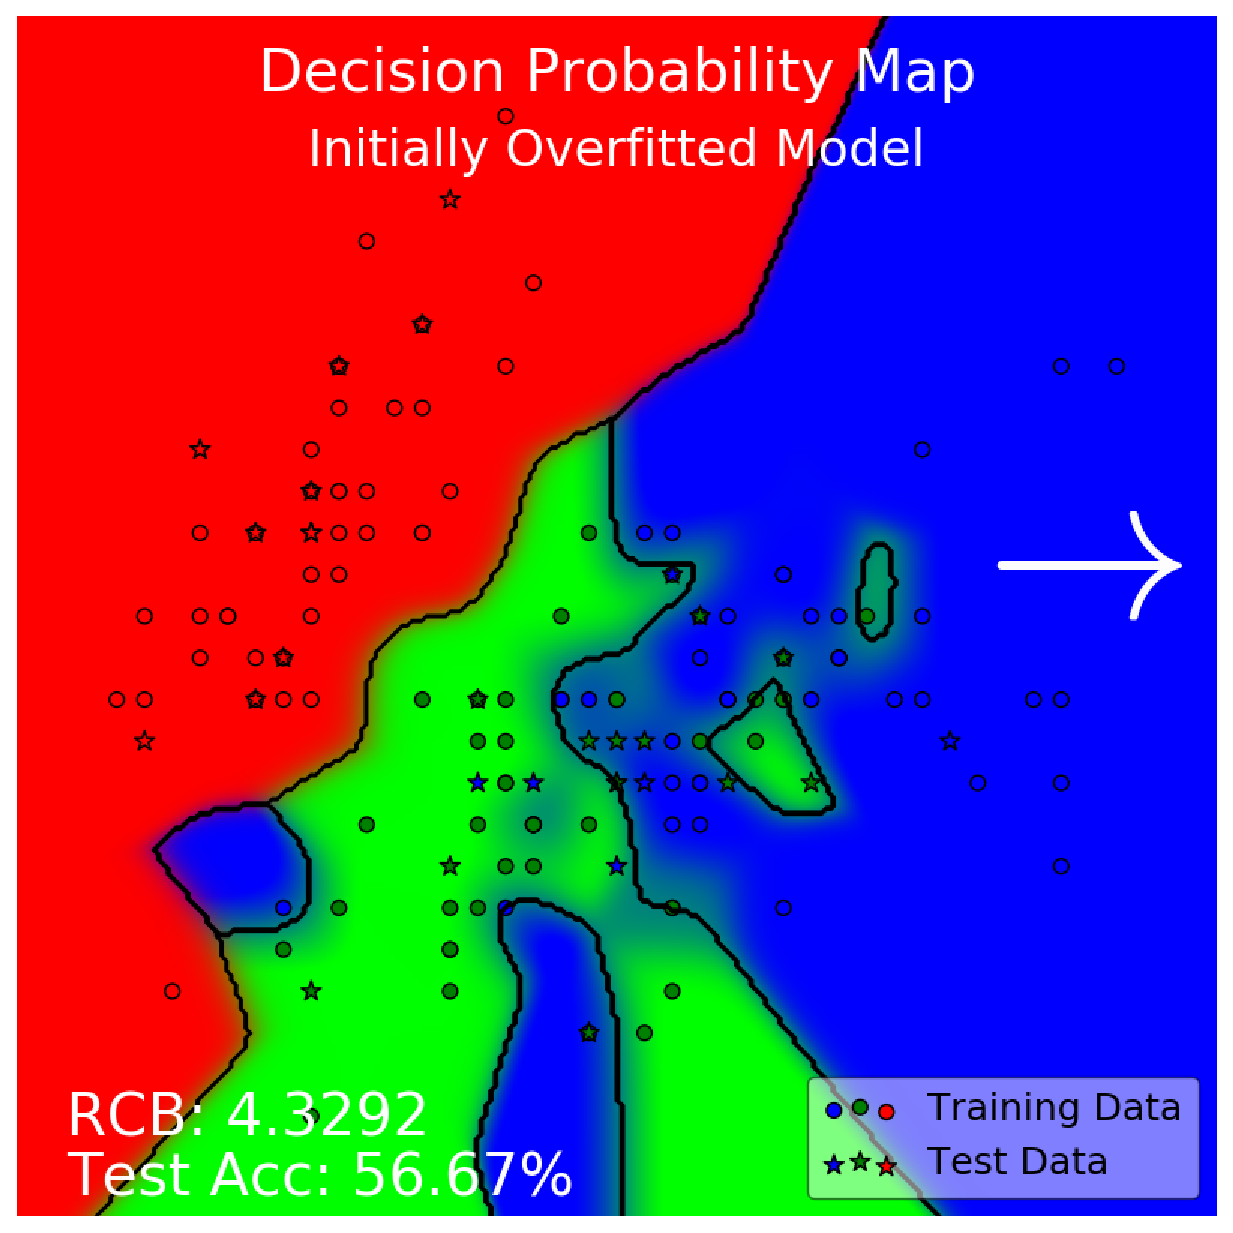
\includegraphics[width=0.32\linewidth]{figures/iris_overfitted_model.eps}
			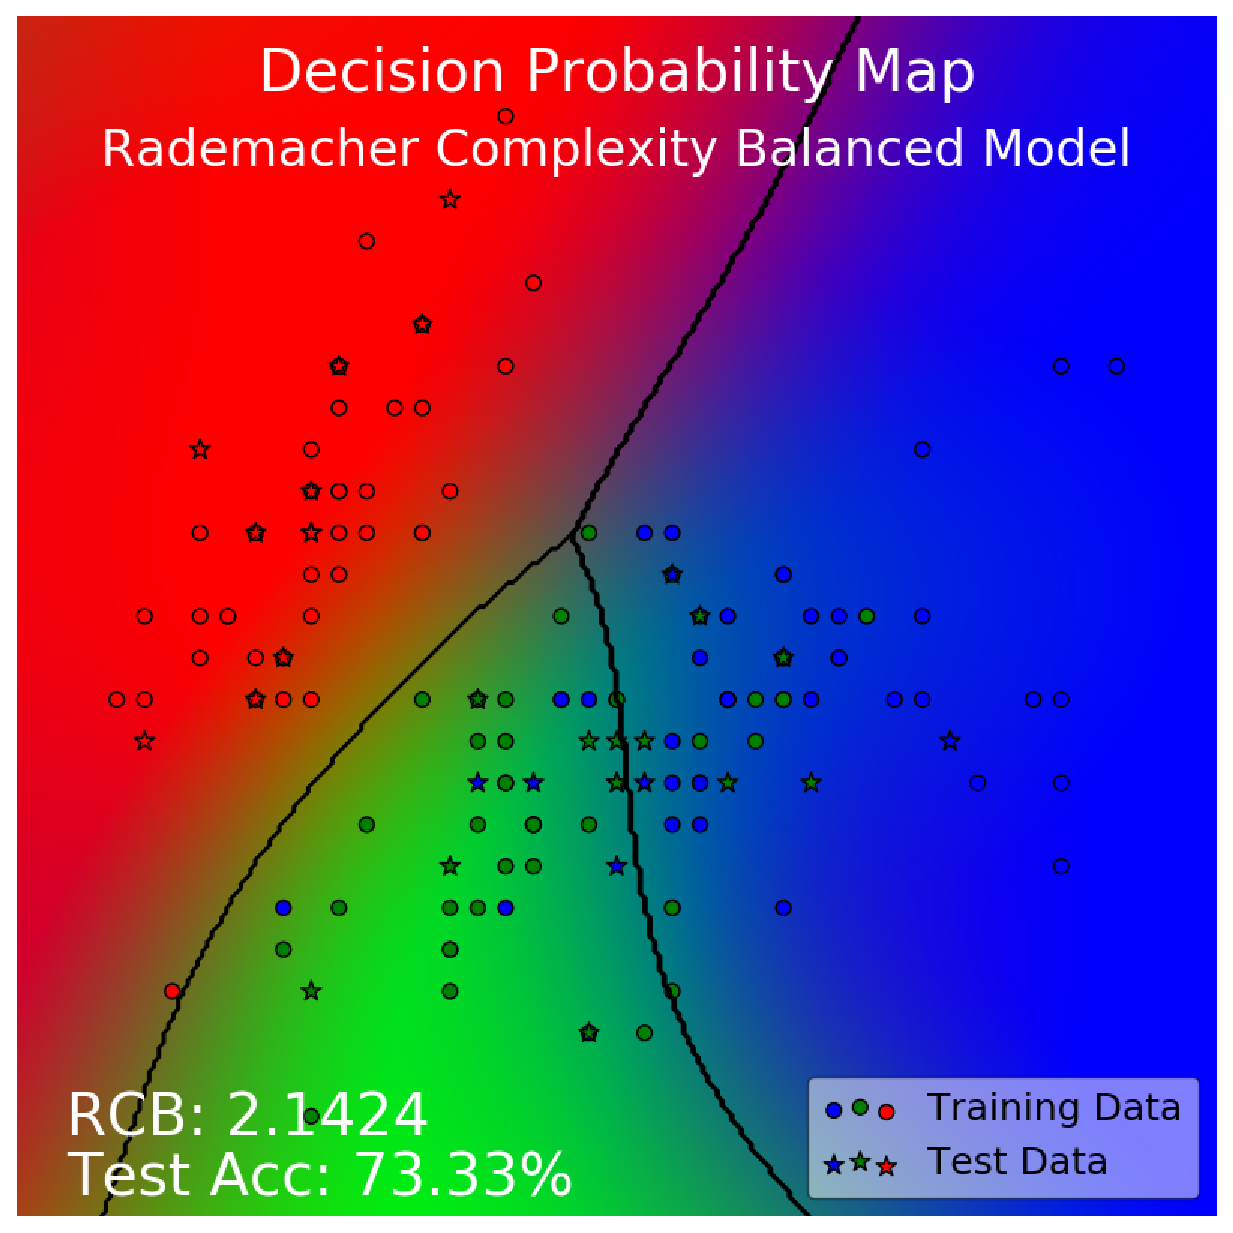
\includegraphics[width=0.32\linewidth]{figures/iris_balanced_model.eps}
			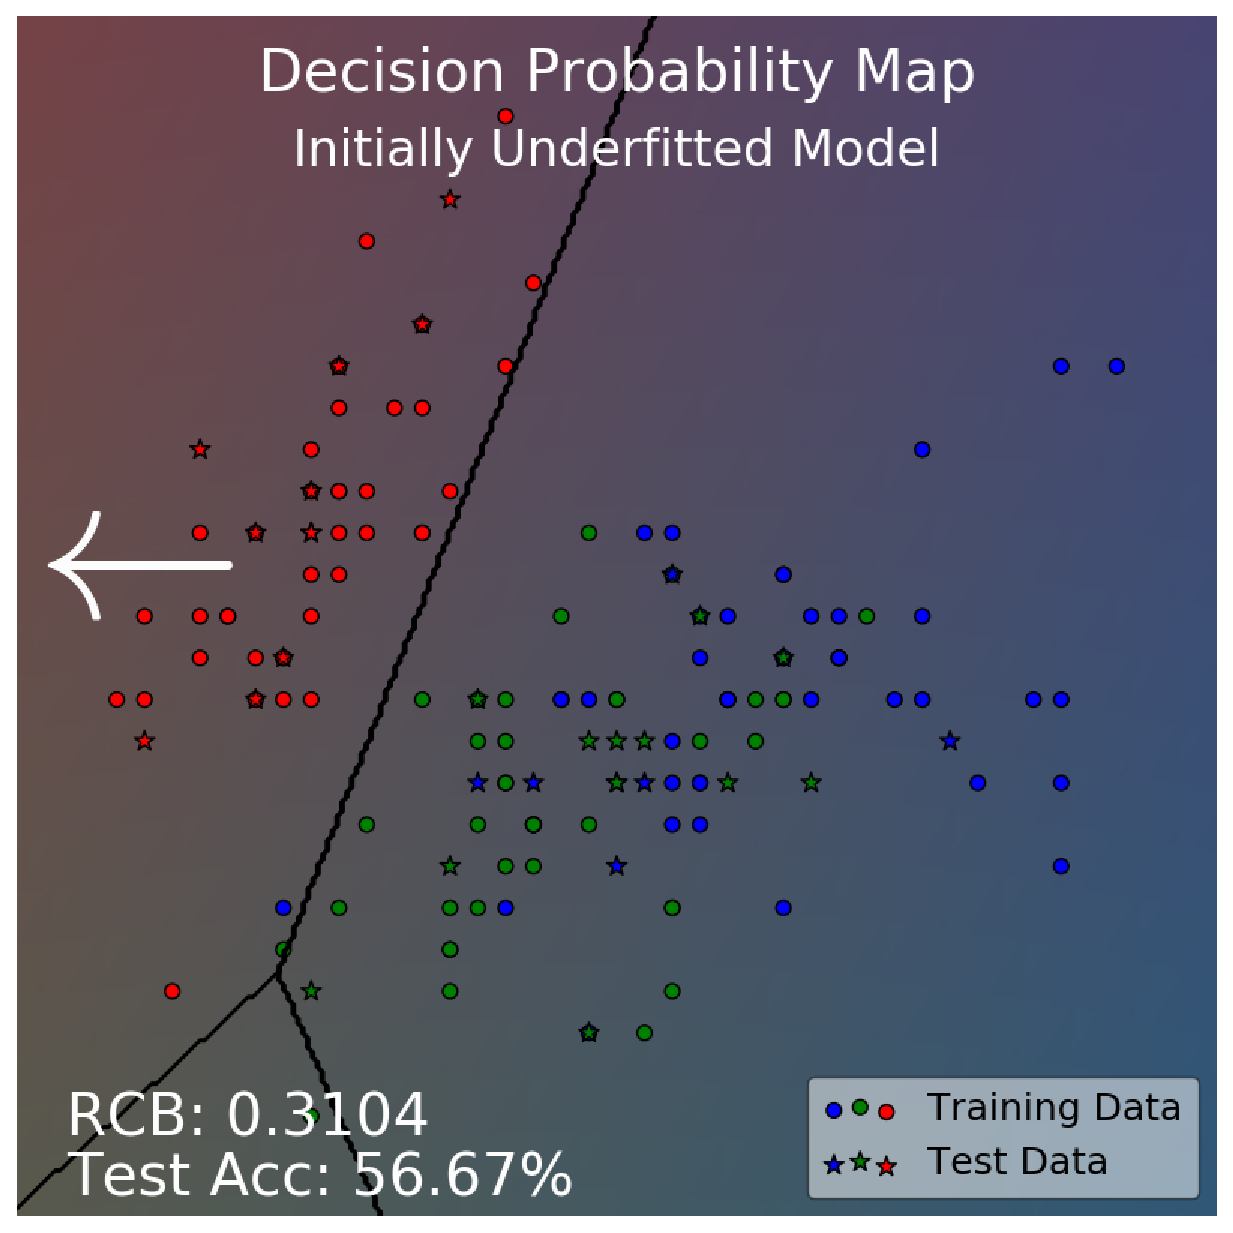
\includegraphics[width=0.32\linewidth]{figures/iris_underfitted_model.eps}
			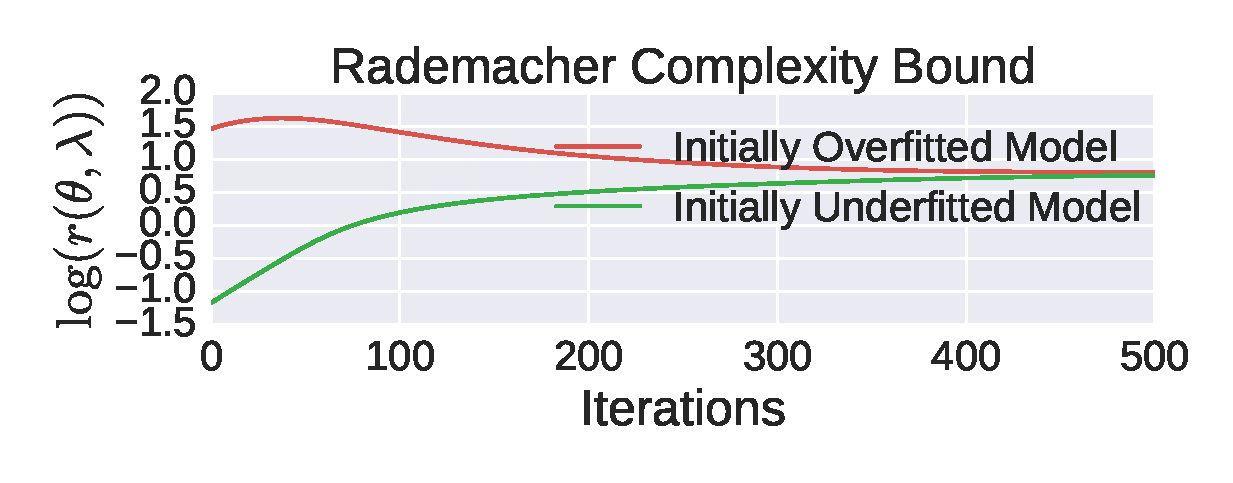
\includegraphics[width=\linewidth]{figures/iris_rademacher_complexity_bound.eps}
			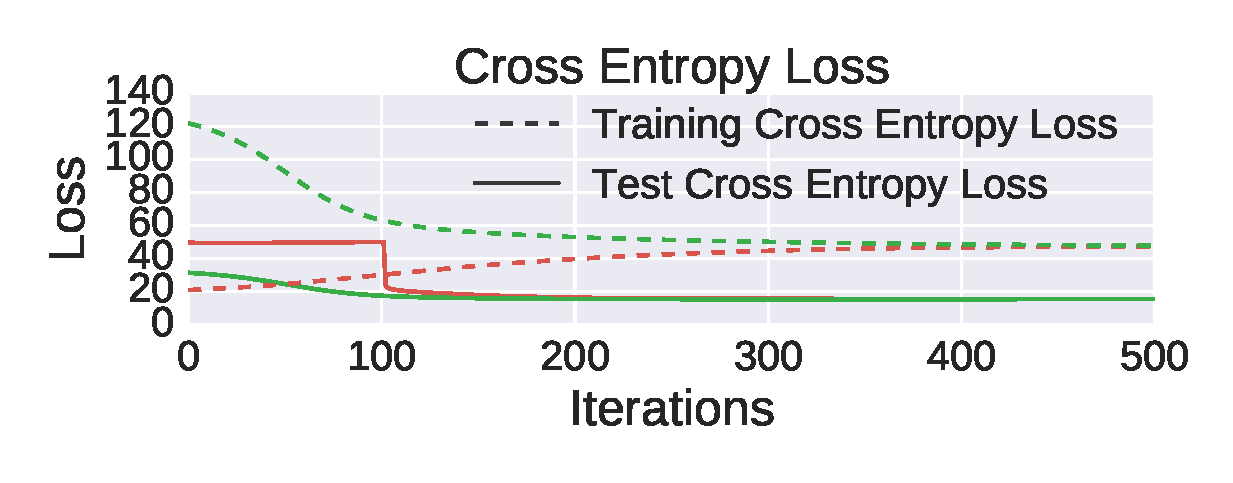
\includegraphics[width=0.48\linewidth]{figures/iris_cross_entropy_loss.eps}
			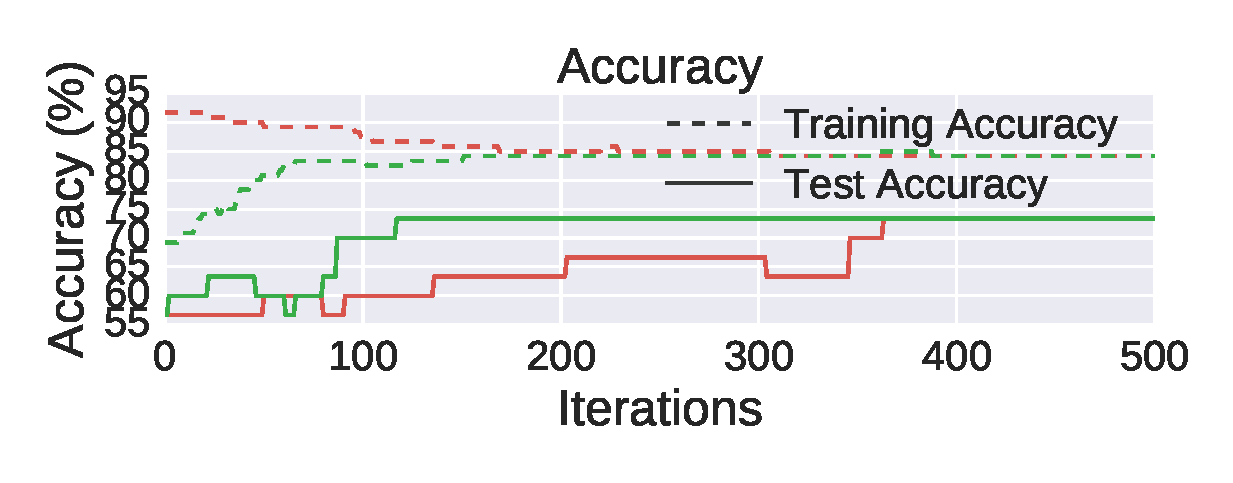
\includegraphics[width=0.48\linewidth]{figures/iris_accuracy.eps}
			\caption{Rademacher complexity balanced learning of hyperparameters for an isotropic Gaussian kernel embedding classifier, using the first two attributes of the iris dataset.}
			\label{fig:iris}
		\end{figure}
		
		The first two of four total attributes of the iris dataset \citep{fisher1936use} is known to have class labels that are not only not linearly separable, but also non-separable by any means, in that the same example $x \in \mathbb{R}^{2}$ may be assigned different output labels $y \in \mathbb{N}_{3} := \{1, 2, 3\}$ as they were only separable with the two remaining attributes. In these difficult scenarios, the notion of model complexity is extremely important, and the success of a learning algorithm greatly depends on how it balances training performance and model complexity to avoid both underfitting and overfitting. 
		
		\Cref{fig:iris} demonstrates \cref{alg:kernel_embedding_classifier_training} with full gradient updates ($n_{b} = n$) to learn hyperparameters of the conditional embedding on the two attribute iris dataset. The kernel used is isotropic Gaussian with diagonal length scales $\Sigma = \ell^{2} I_{2}$ and sensitivity $\alpha = \sigma_{f}$, so the hyperparameters are $\theta = (\alpha, \ell)$ and $\lambda$. We evaluate the performance of the learning algorithm on a withheld test set using 20\% of the available 150 data samples. Attributes are scaled into the unit range $[0, 1]$ and decision probability maps are plotted for the region $[-0.5, 1.05]^{2}$, where the red, green, and blue colour channels represent the clip-normalised decision probability \eqref{eq:empirical_decision_probability_clip_normalised} for classes $c = 1, 2, 3$. We begin from two initial scenarios, one originally overfitting ($\alpha_{o} = 0.01$, $\ell_{o} = 0.035$, $\lambda_{o} = 10^{-6}$) and another underfitting ($\alpha_{u} = 1$, $\ell_{u} = 1$, $\lambda_{u} = 1$) the training data. Initially, both models performs sub-optimally with a test accuracy of 56.67\%. We see that the Rademacher complexity bound (RCB) $r(\theta, \lambda)$ appropriately measures the amount of overfitting with $r((\alpha_{o}, \ell_{o}), \lambda_{o}) = 4.33$ and $r((\alpha_{u}, \ell_{u}), \lambda_{u}) = 0.31$. We then learn model hyperparameters with \cref{alg:kernel_embedding_classifier_training} for 500 iterations from both initialisations at rate $\eta = 0.01$, where both models converges to a balanced model with appropriate complexity bounds $r((\alpha_{o}, \ell_{o}), \lambda_{o}) = r((0.01, 0.24), 8.62 \times 10^{-7}) = 2.23 \approx 2.14 = r((\alpha_{u}, \ell_{u}), \lambda_{u}) = r((5.1, 0.24), 0.20)$ and an improved test accuracy of 73.33\%. In particular, the initially overfitted model learns a simpler model at the expense of lower training performance, emphasising the benefits of complexity based regularisation, without which the learning would only maximise training performance at the cost of further overfitting. Meanwhile, the initially underfitted model learns to trade some complexity away to improve the unflattering performance on the training set. In both scenarios, our learning algorithm improved performance on the test set.
		
	\paragraph{UCI Datasets}
	
		\begin{table}[t]
			\caption{Classification accuracy (\%) of kernel embedding classifiers on UCI datasets}
			\label{tab:uci_experiments}
			\centering
			\begin{tabular}{lccccc}			
				Dataset \hspace{\fill} $(n, d, m)$ & GKEC & GKEC-SGD & KEN-1 & KEN-2 & Others \\
				\midrule
				\texttt{banknote} \hspace{\fill} (1372, 4, 2) & $99.9 \pm 0.2$ & $98.8 \pm 0.9$ & $99.5 \pm 1.0$ & $99.4 \pm 0.9$ & 99.78\textsuperscript{a} \\
				\texttt{ecoli} \hspace{\fill} (336, 7, 8) & $87.5 \pm 4.4$ & $84.5 \pm 5.0$ & $87.5 \pm 3.2$ & $86.3 \pm 6.0$ & 81.1\textsuperscript{b} \\
				\texttt{robot} \hspace{\fill} (5456, 24, 4) & $96.7 \pm 0.9$ & $95.5 \pm 0.9$ & $82.3 \pm 7.1$ & $94.5 \pm 0.8$ & 97.59\textsuperscript{c} \\
				\texttt{segment} \hspace{\fill} (2310, 19, 7) & $98.4 \pm 0.8$ & $96.1 \pm 1.5$ & $94.6 \pm 1.6$ & $96.7 \pm 1.1$ & 96.83\textsuperscript{d} \\
				\texttt{wine} \hspace{\fill} (178, 13, 3) & $97.2 \pm 3.7$ & $93.3 \pm 6.0$ & $96.1 \pm 5.0$ & $97.2 \pm 5.1$ & 100\textsuperscript{e} \\
				\texttt{yeast} \hspace{\fill} (1484, 8, 10) & $52.5 \pm 2.1$ & $60.3 \pm 4.4$ & $55.8 \pm 5.0$ & $59.6 \pm 4.0$ & 55.0\textsuperscript{b} \\
			\end{tabular}
		\end{table}
		
		We demonstrate the average performance of learning anisotropic Gaussian kernels and kernels with explicit neural network features on standard UCI datasets \citep{bache2013uci}, summarised in \cref{tab:uci_experiments}. The former has a shallow but wide model architecture, while the latter has a deeper but narrower model architecture. The Gaussian kernel is learned with both full (GKEC) and batch stochastic gradient updates (GKEC-SGD) using a tenth ($n_{b} \approx \frac{n}{10}$) of the training set each training iteration, with sensitivity and length scales initialised to $1$. For neural network induced kernels, we randomly select two simple fully connected architectures with 16-32-8 (KEN-1) and 96-32 (KEN-2) hidden units respectively, and learn the conditional embedding without dropout under ReLU activation. Biases and standard deviations of zero mean truncated normal distributed weights are initialised to $0.1$, and are to be trained with full gradient updates. For all experiments, $\lambda$ is initialised to $1$ and is learned jointly with the kernel. Classifiers are trained with the Adam optimiser \citep{kingma2014adam} in TensorFlow \citep{abadi2016tensorflow} with rate $\eta = 0.1$ and $\epsilon = 10^{-15}$ under the learning objective $q(\theta, \lambda)$ \eqref{eq:learning_objective}. Training is ran for 1000 or 10000 iterations when using full or batch gradient updates respectively, regardless of convergence. All attributes are scaled to the unit range. Each classifier is trained on 9 out of 10 folds and tested on the remaining fold, which are shuffled over all 10 combinations to obtain the test accuracy average and deviation. We compare our results to other approaches using neural networks \citep[a; c]{kaya2016banknote, freire2009short}, probabilistic binary trees \citep[b]{horton1996probabilistic}, decision trees \citep[d]{zhou2004size}, and regularised discriminant analysis \citep[e]{aeberhard1992comparison}. \Cref{tab:uci_experiments} shows that our learning algorithm achieves similar performance without any special tuning or heuristics, but by simply placing a conditional embedding on training data and applying a complexity bound based learning algorithm. The SGD approach for Gaussian kernels performs similarly to the full gradient approach, supporting \cref{thm:expected_risk_bound_hyperparameter_learning_copy} for $n = n_{b}$. For neural network features, we did not attempt to choose an optimal architecture for each dataset. The learning algorithm is to train the same simple untrained network for different datasets under only 1000 iterations, and still generates comparable performance. 
	
	\paragraph{MNIST by learning pixel length scales}
	
		We apply \cref{alg:kernel_embedding_classifier_training} to learn anisotropic length scales of Gaussian kernels on pixels of the MNIST digits dataset \citep{lecun1998gradient}. We first demonstrate the test performance of KECs as the training set increases in size, verifying \cref{thm:probability_convergence_copy} in that decision probabilities converge to the true and thus test distribution as $n$ increases. In the top left plot of \cref{fig:mnist_experiments}, we train on datasets of varying sizes, from 50 to 5000 samples, and benchmark performance on the standard test set of 10000 examples. All hyperparameters are initialised to 1 before training. For each $n$, we see that KECs outperform SVCs, since SVCs are unable to learn the length scales of the Gaussian kernel. This also shows that KECs perform very well with small datasets even when $n < d$. The MNIST dataset has $d = 28^{2} = 784$ pixel dimensions, yet with only $n = 50, 150, 250$ training samples, the KEC achieves a test accuracy of 45.7\%, 70.09\%, and 79.37\% respectively, compared to 18.13\%, 37.43\%, and 53.81\% from SVCs. We also compare training under the learning objective with and without the Rademacher complexity bound. For small $n$ below 750 samples, the latter outperforms the former (e.g. 86.69\% and 86.96\% for $n = 500$), while for large $n$ the former outperforms the latter (e.g. 96.05\% and 95.3\% for $n= 5000$). This verifies that complexity based regularisation becomes especially important when data size grows, where overfitting starts to hurt generalisation performance. Our bound is also tighter with larger $n$, so that generalisation performance improves with more data. The images at the bottom of \cref{fig:mnist_experiments} show the pixel length scales learned through batch stochastic gradient updates ($n_{b} = 1200$) on all available training images of the digits indicated, demonstrating the most discriminative regions for classification. In particular, the most discriminative regions are usually around the edges of the digits, subject to slight intraclass translations. 
		
	\paragraph{MNIST by learning convolutional features}
	
		\begin{figure}[t]
			\centering 
			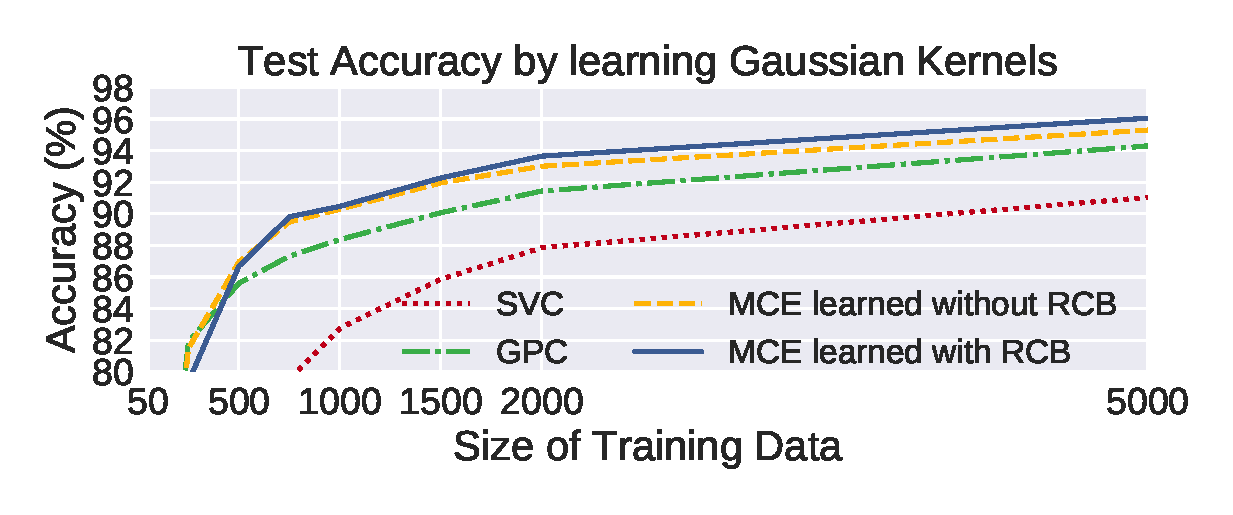
\includegraphics[width=0.49\linewidth]{figures/gaussian_mnist_test_performance_short.eps}
			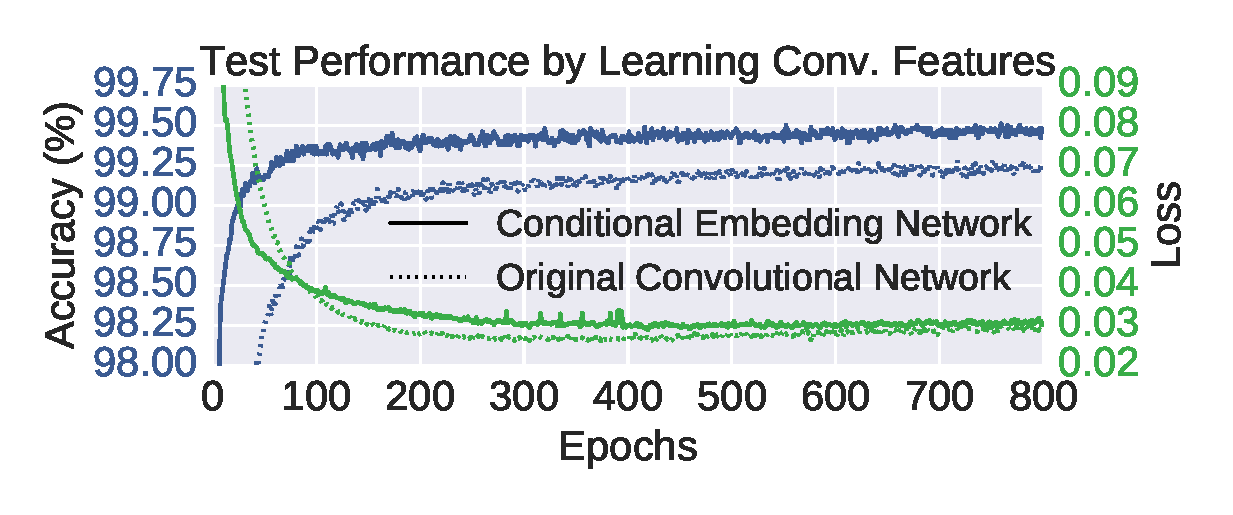
\includegraphics[width=0.49\linewidth]{figures/deep_mnist_test_performance_short.eps}
			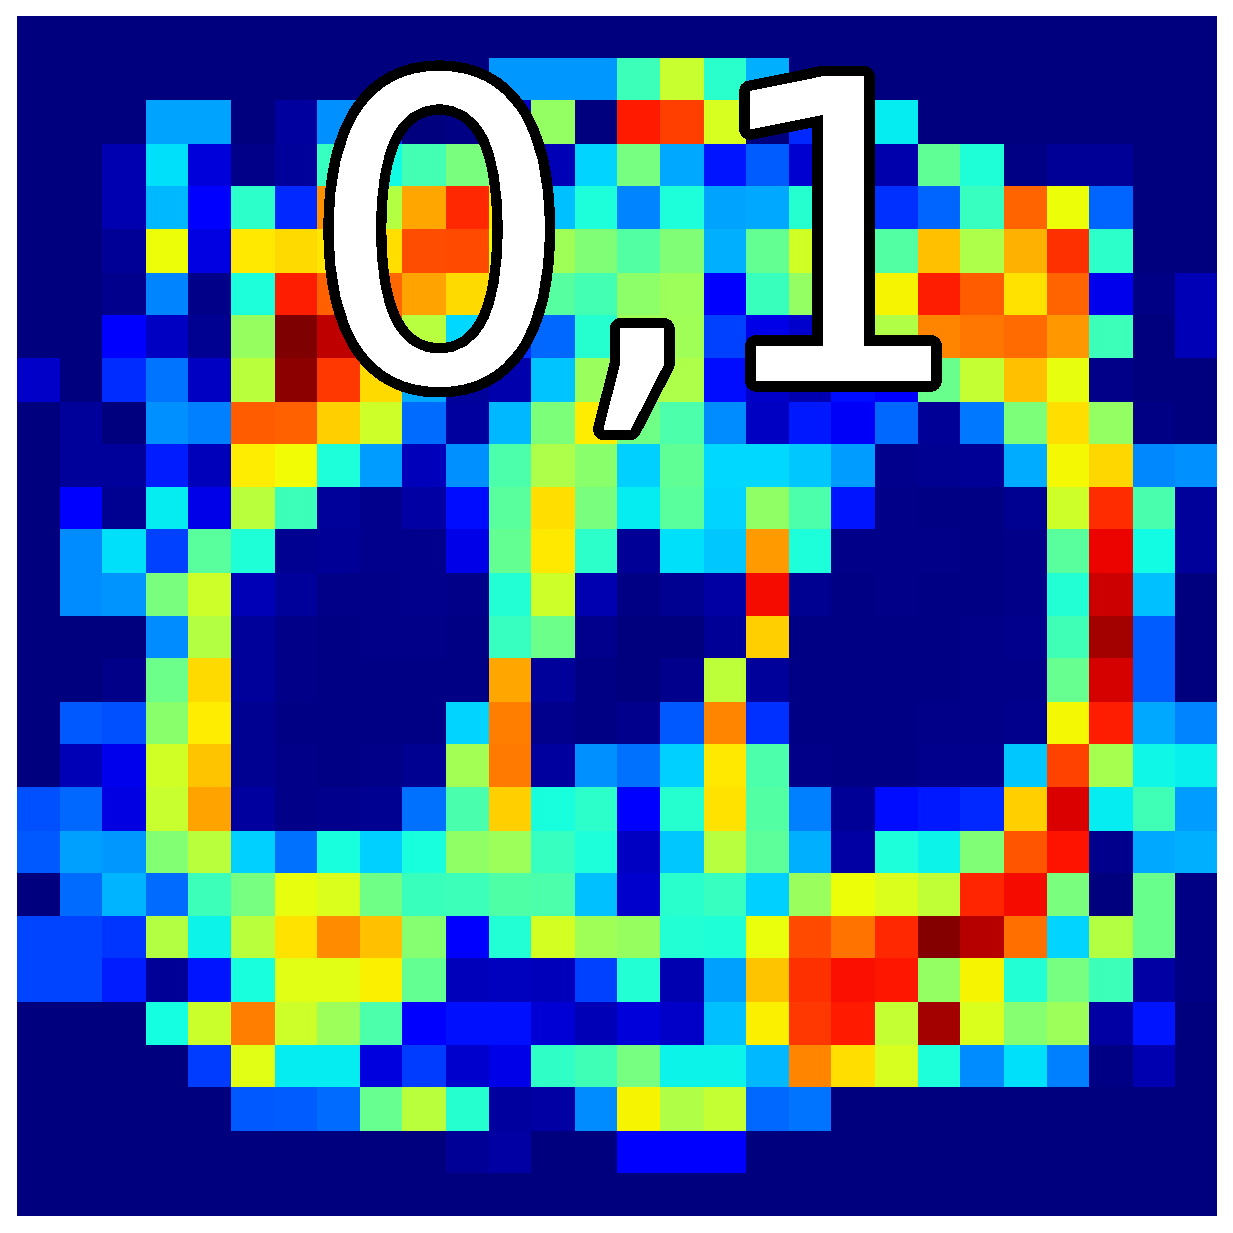
\includegraphics[width=0.1\linewidth]{figures/pixel_relevance_01_batch_1200.eps}
			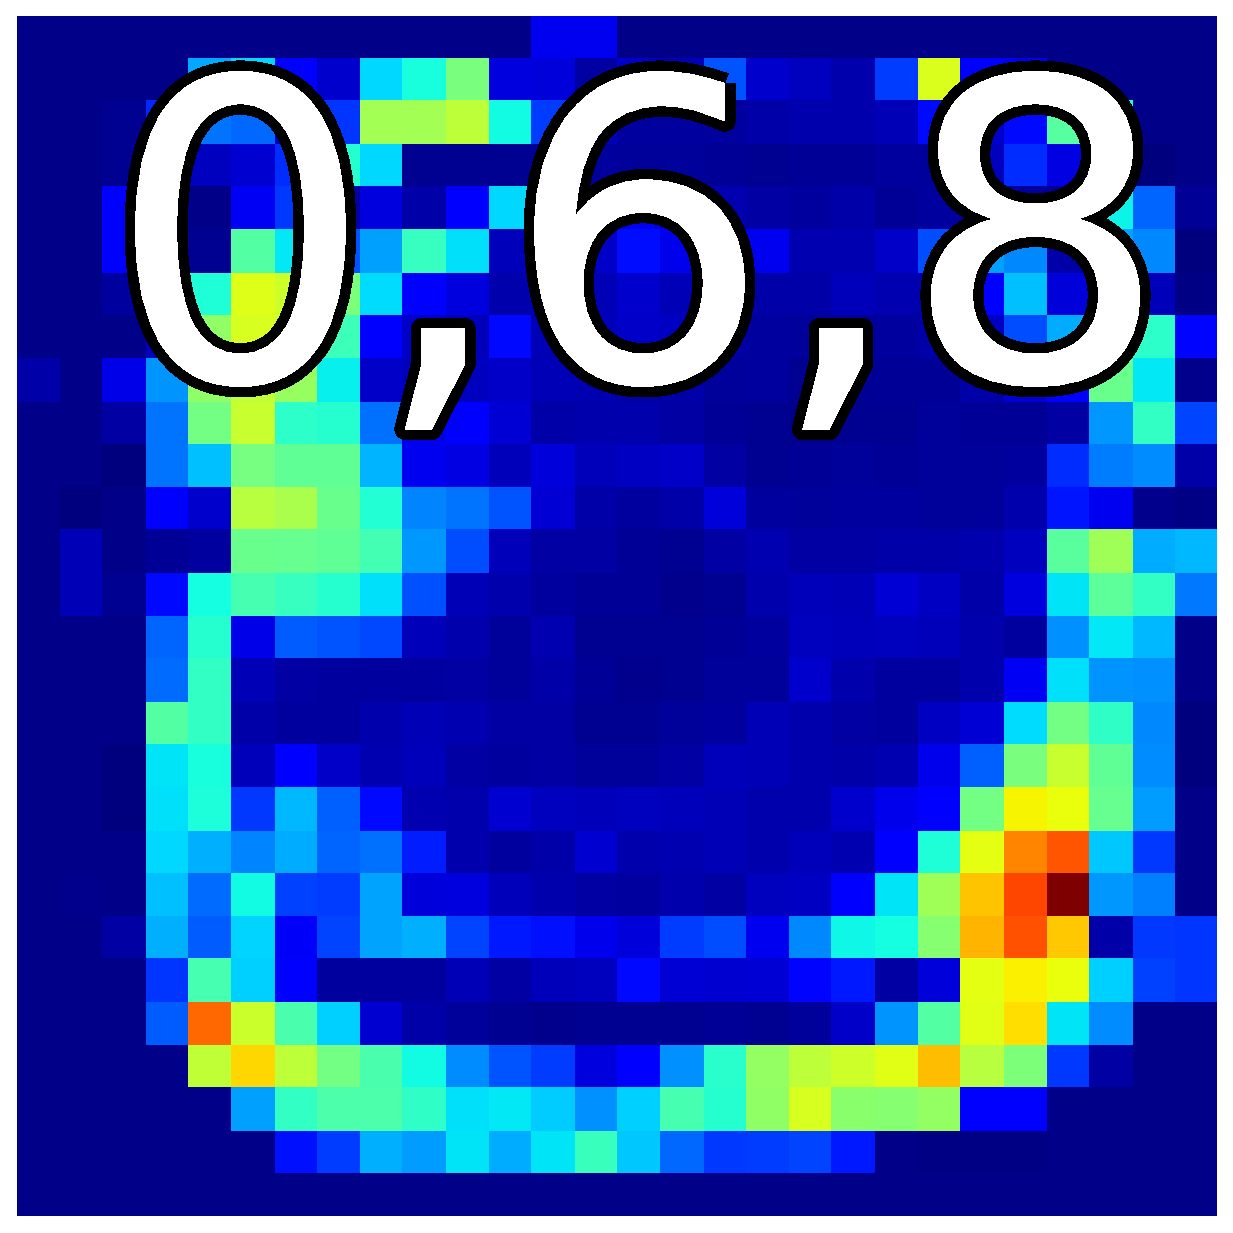
\includegraphics[width=0.1\linewidth]{figures/pixel_relevance_068_batch_1200.eps}
			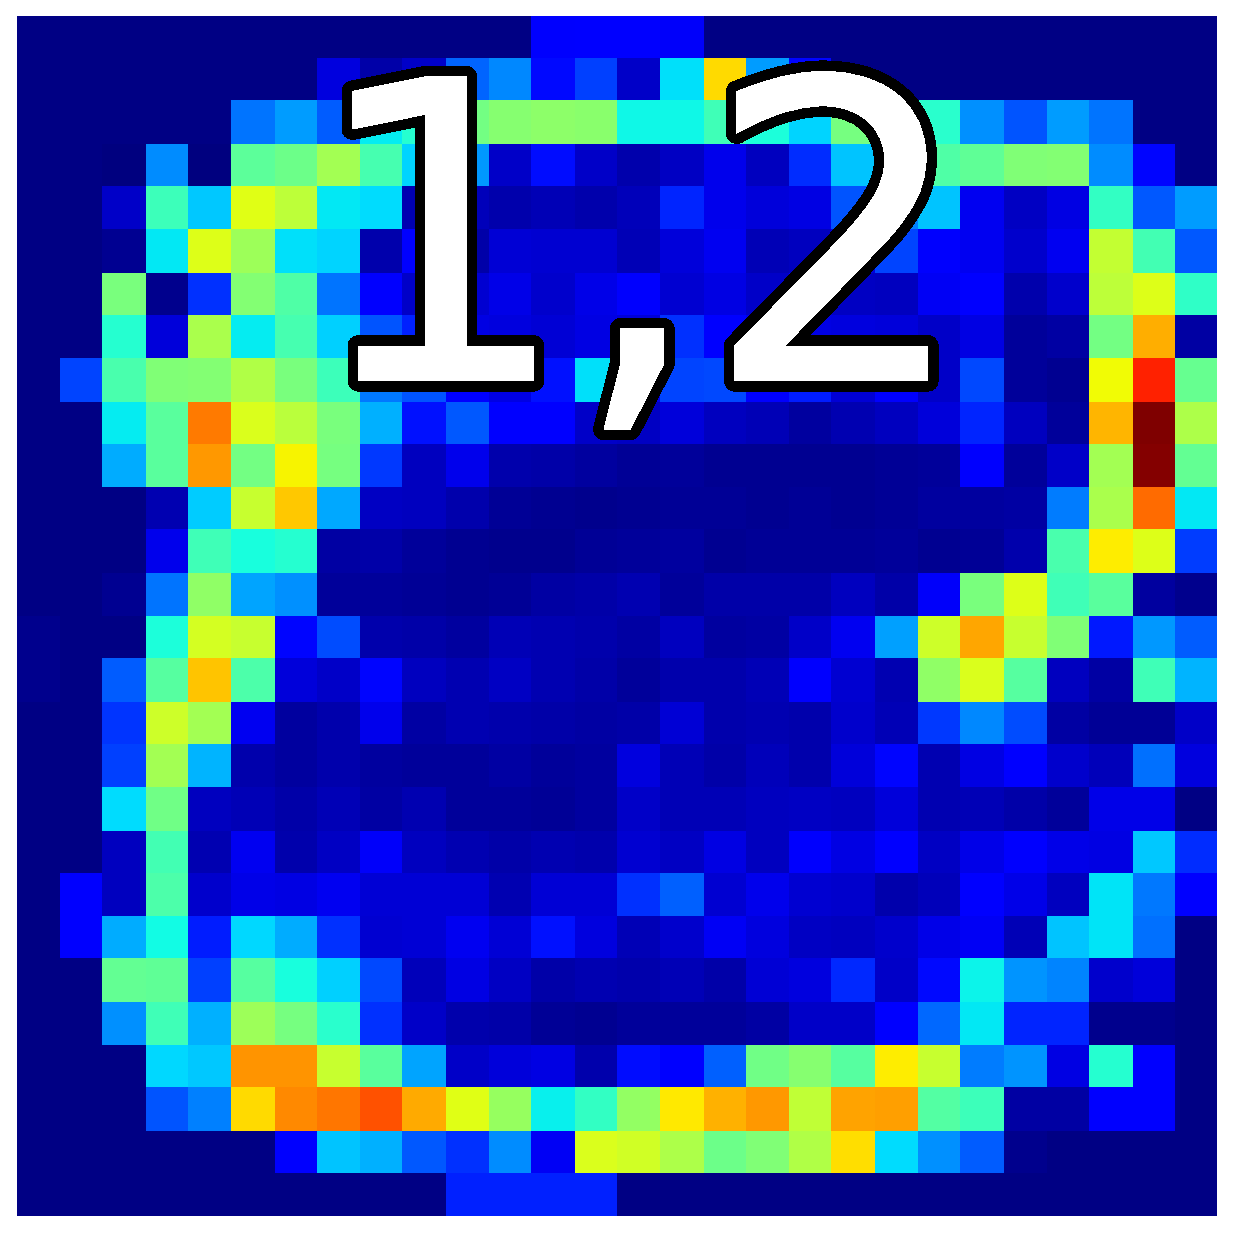
\includegraphics[width=0.1\linewidth]{figures/pixel_relevance_12_batch_1200.eps}
			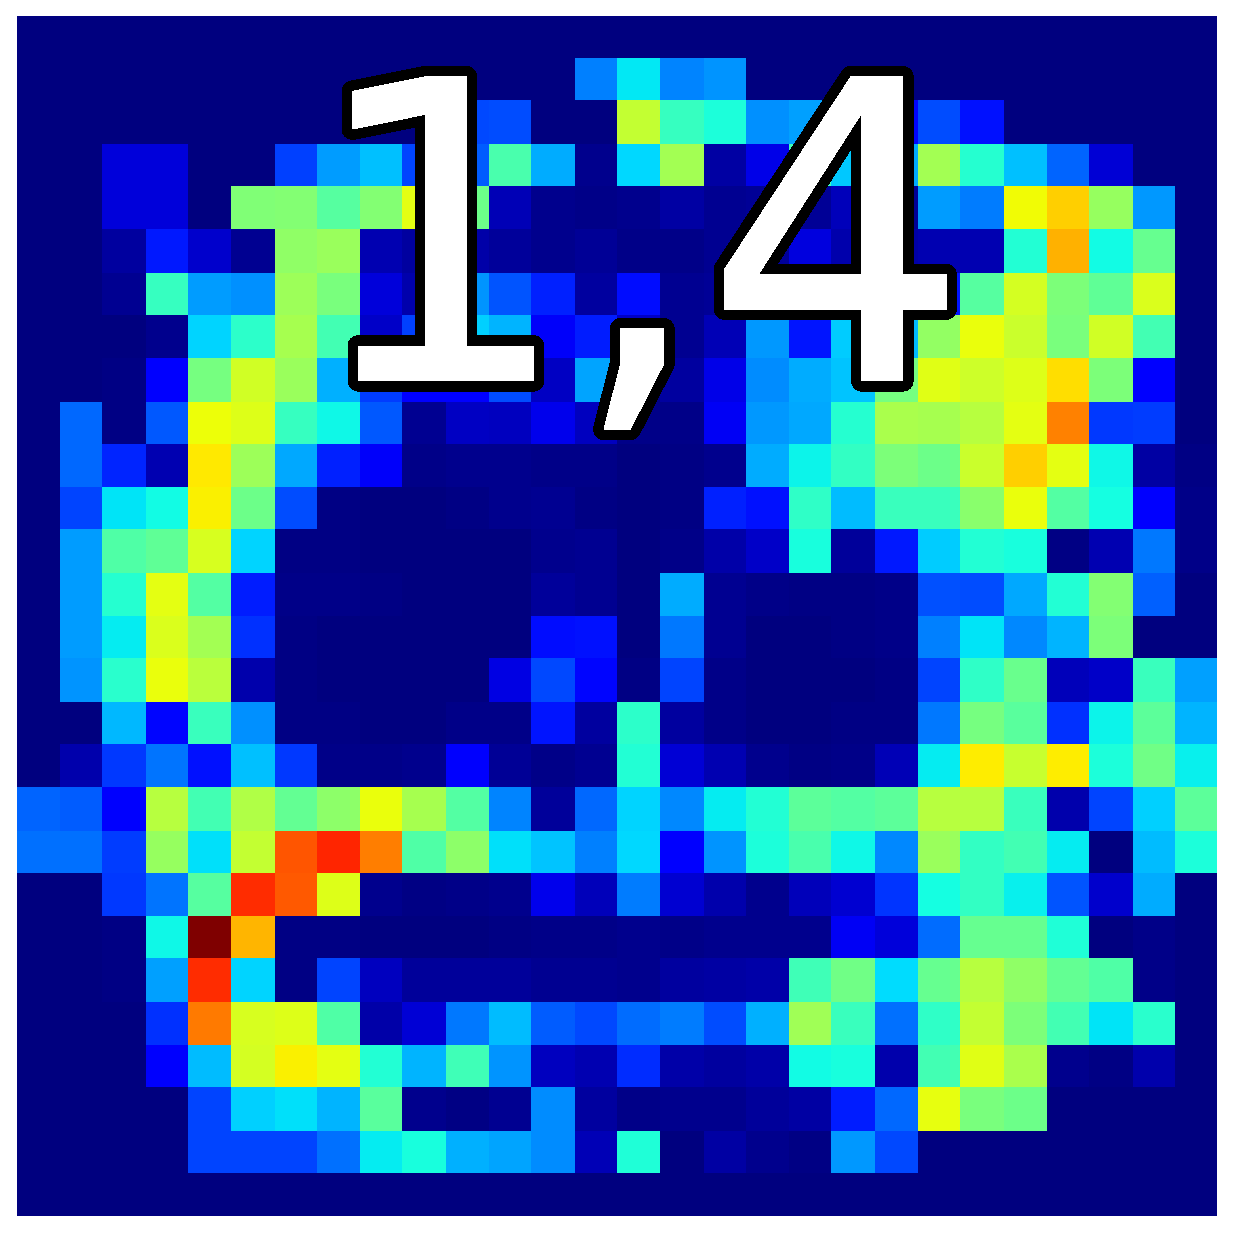
\includegraphics[width=0.1\linewidth]{figures/pixel_relevance_14_batch_1200.eps}
			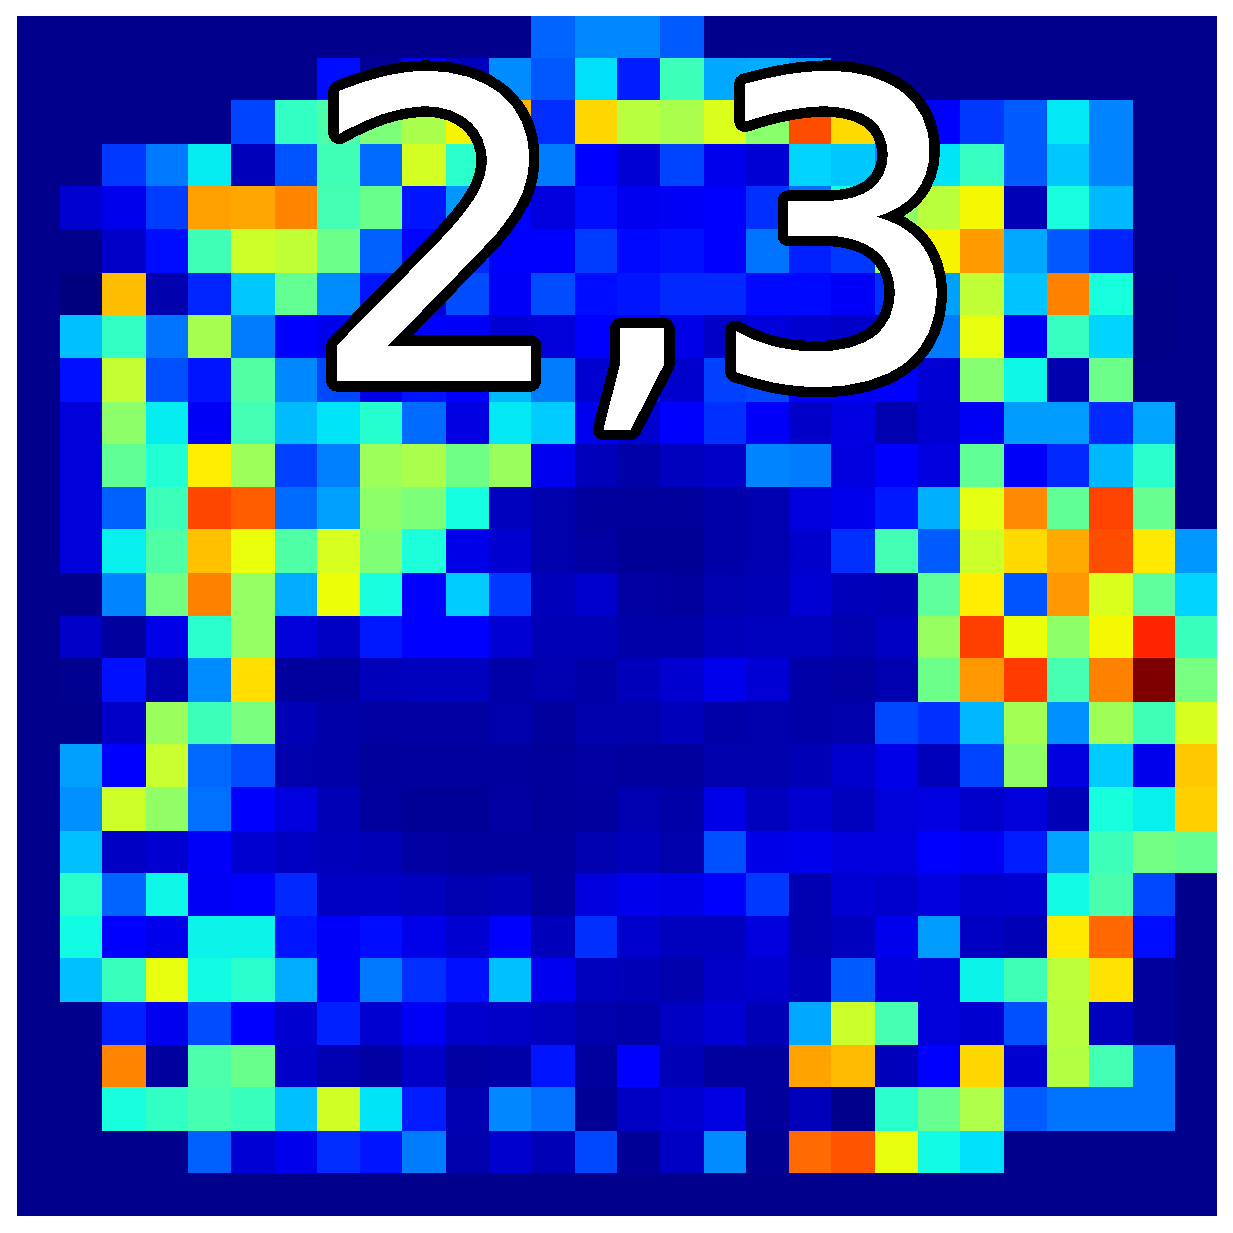
\includegraphics[width=0.1\linewidth]{figures/pixel_relevance_23_batch_1200.eps}
			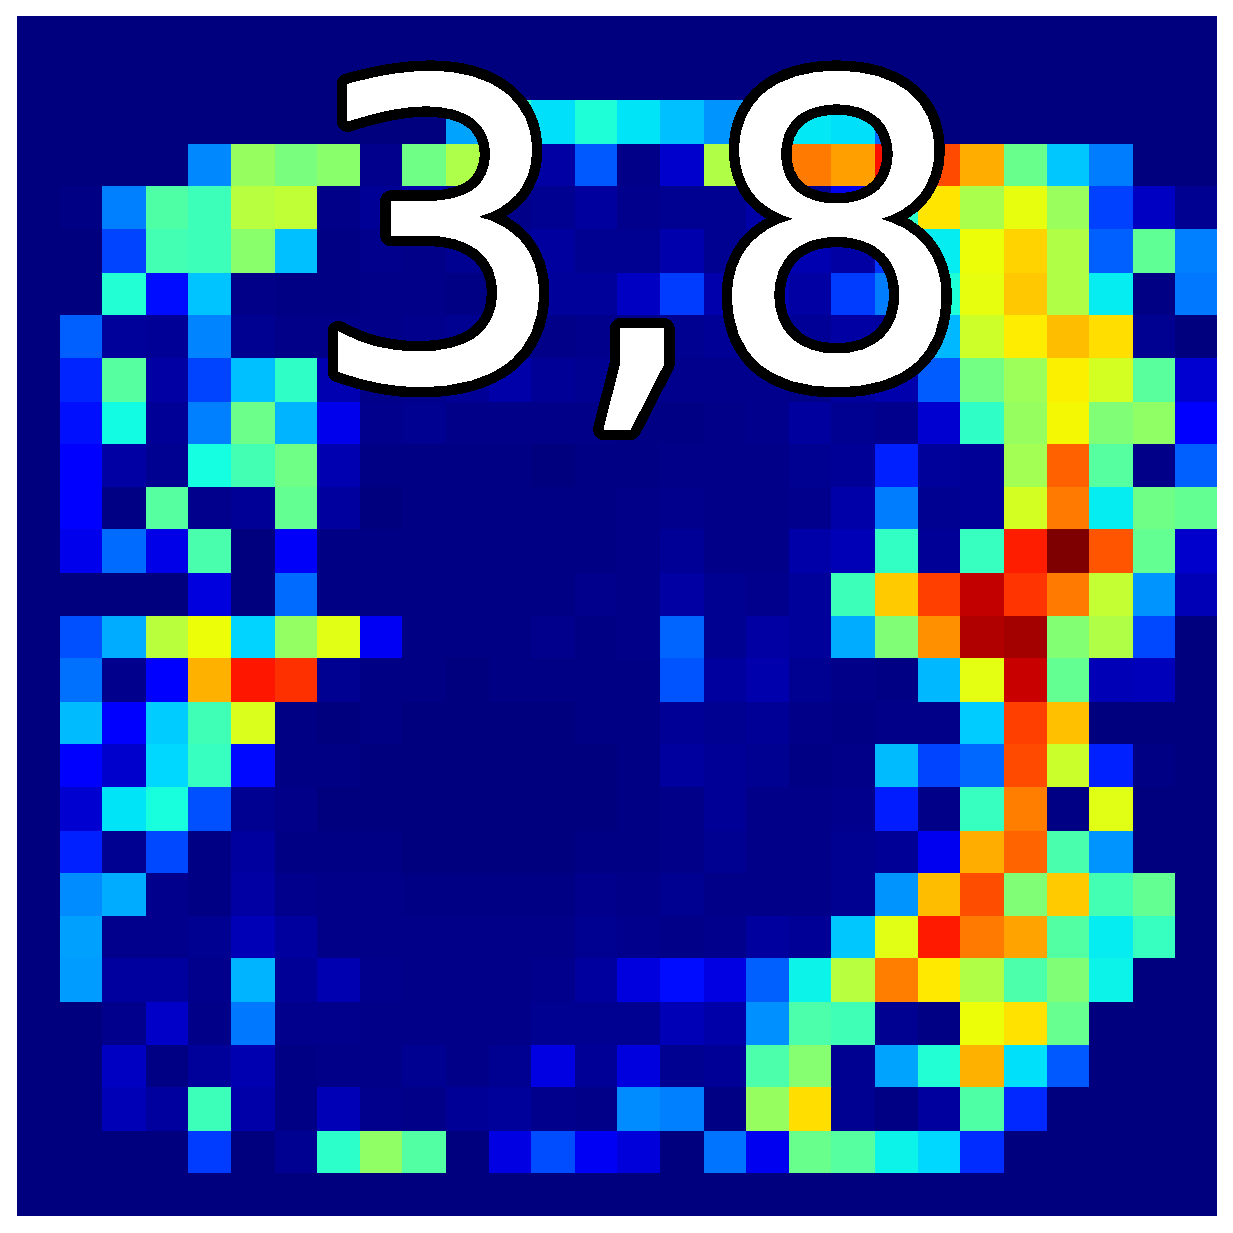
\includegraphics[width=0.1\linewidth]{figures/pixel_relevance_38_batch_1200.eps}
			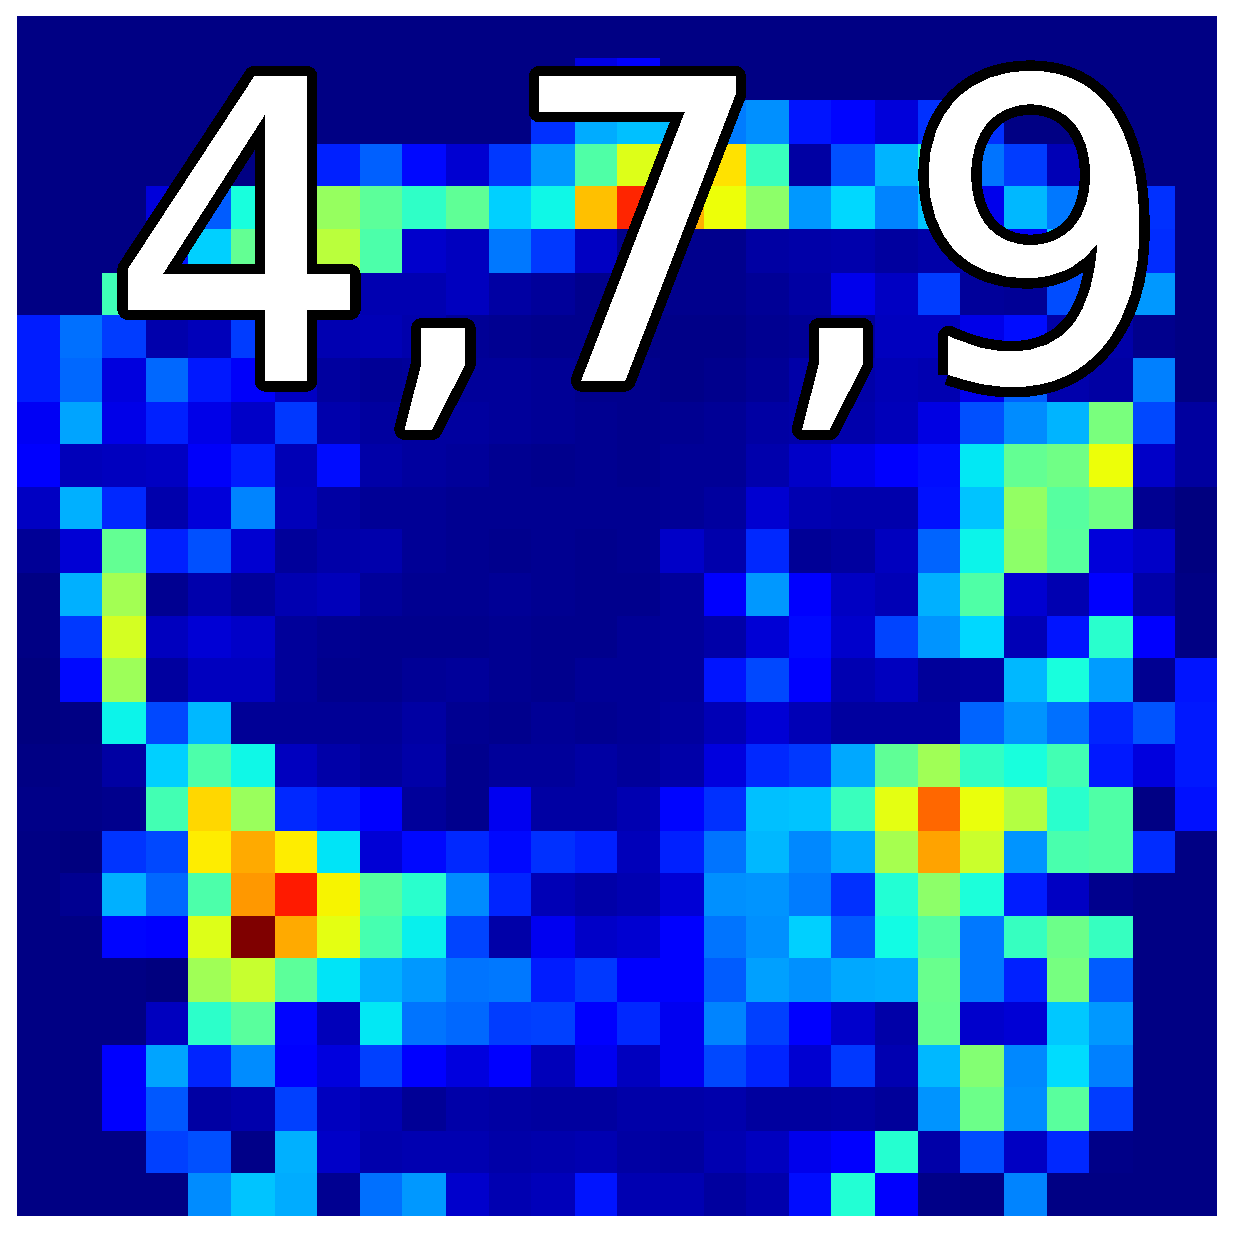
\includegraphics[width=0.1\linewidth]{figures/pixel_relevance_479_batch_1200.eps}
			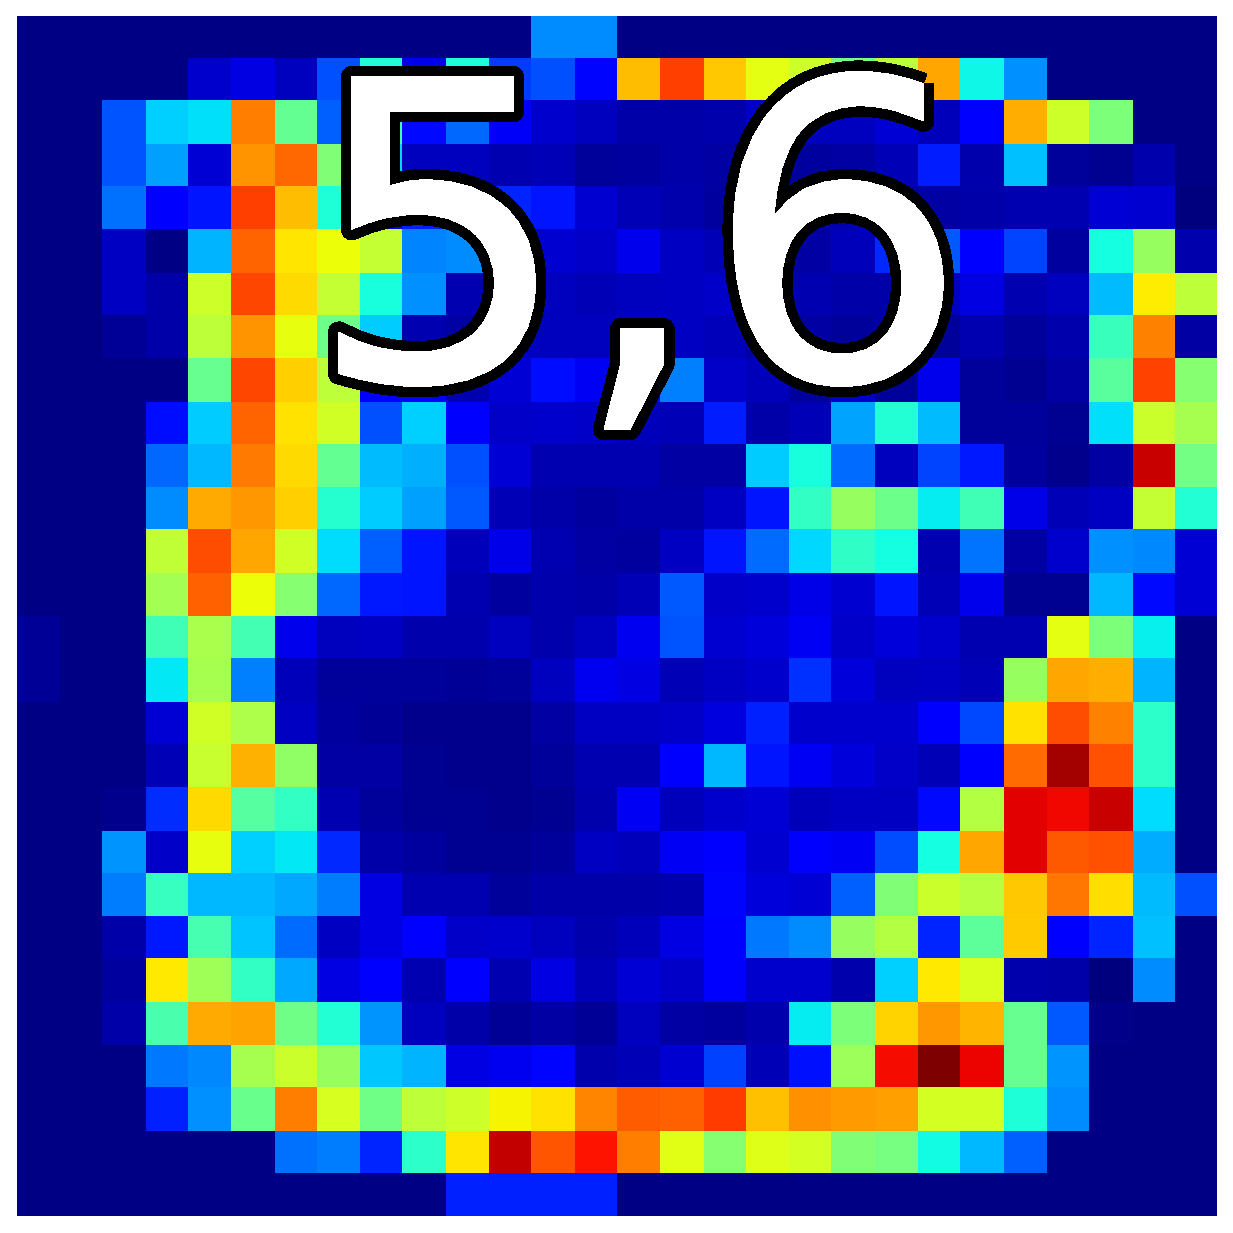
\includegraphics[width=0.1\linewidth]{figures/pixel_relevance_56_batch_1200.eps}
			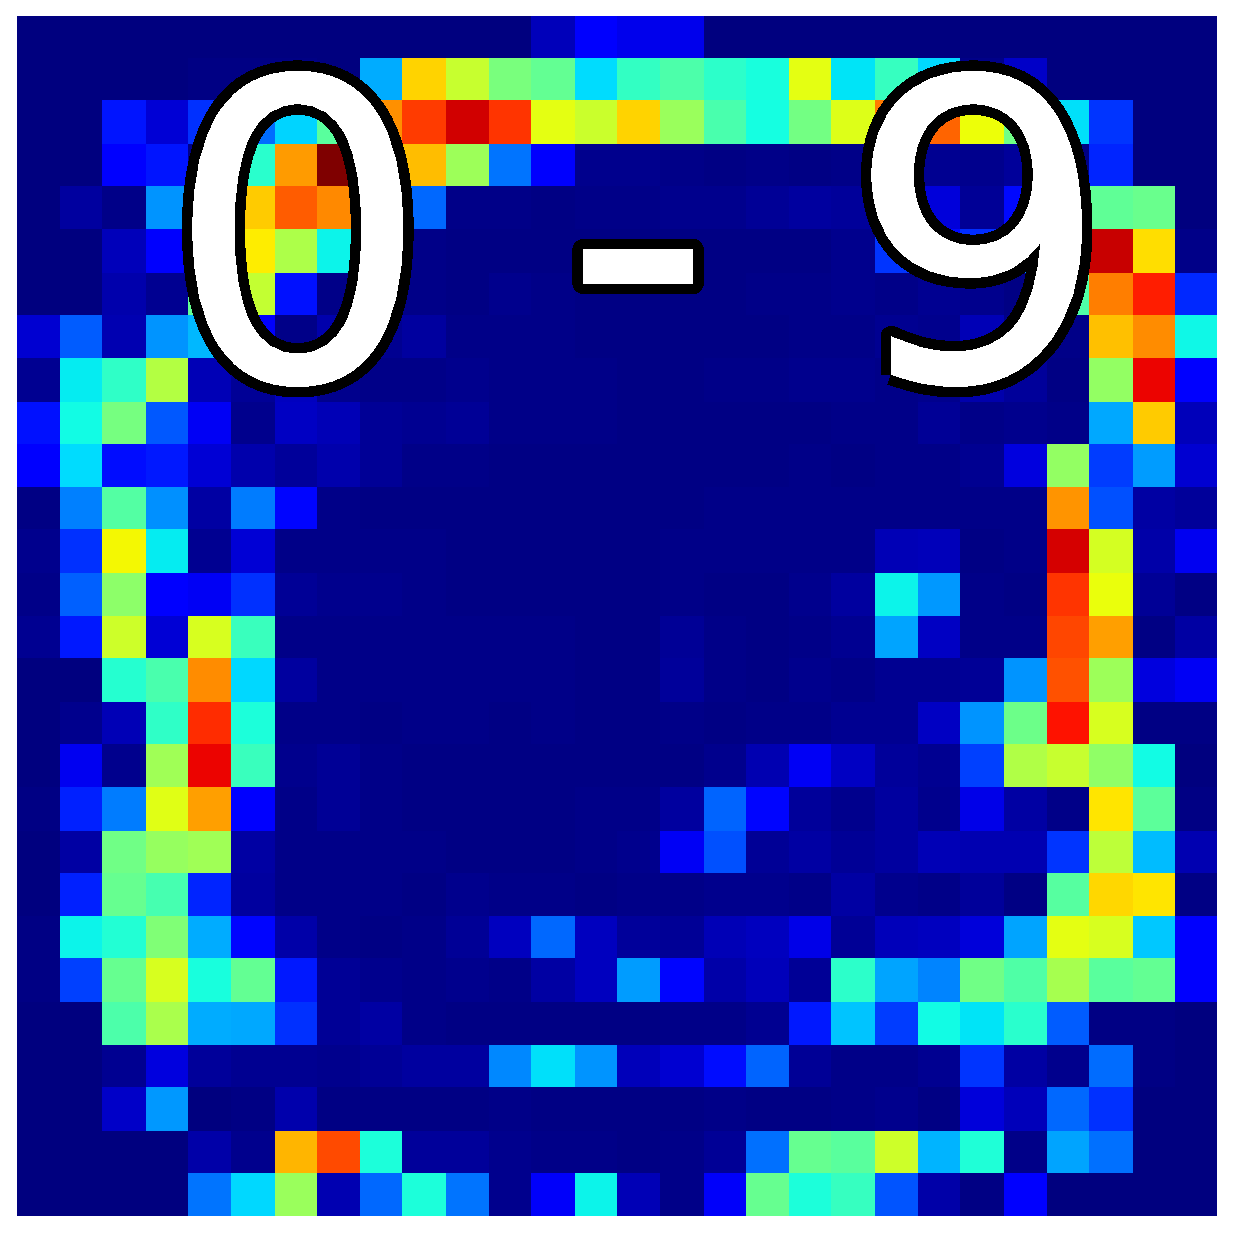
\includegraphics[width=0.1\linewidth]{figures/pixel_relevance_0123456789_batch_1200.eps}
			\caption{Top: Test accuracy and cross entropy loss by learning Gaussian kernels (left) and deep convolutional features (right). Bottom: Learned pixel length scales under Gaussian kernels.}
			\label{fig:mnist_experiments}
		\end{figure}
		
		We now apply our learning algorithm to train convolutional neural networks (CNN) on the MNIST dataset. We employ an example architecture from the TensorFlow tutorial on deep MNIST classification \citep{abadi2016tensorflow}. This ReLU activated architecture uses two convolutional layers, each with max pooling, followed by a fully connected layer with a drop out probability of 0.5. The original network then employs a final softmax regressor on the last hidden layer for classification. The kernel embedding network instead employs a linear kernel on the last hidden layer to construct the conditional embedding. We then train both networks from the same initialisation with stochastic gradient updates using $n_{b} = 6000$ images at a time for 800 epochs, with learning rate $\eta = 0.01$. All biases and standard deviations of zero mean truncated normal distributed weights are initialised to 0.1. The convolutional features of the kernel embedding network are trained jointly with the regularisation parameter, initialised to $\lambda = 10$, under our proposed learning objective \eqref{eq:learning_objective}, while the original CNN is trained under its usual cross entropy loss. The fully connected layer is trained with a drop out probability of 0.5 for both cases to allow direct comparison. The top right plot in \cref{fig:mnist_experiments} shows that kernel embedding networks learn convolutional features at a much faster rate, maintaining a higher test accuracy at all epochs. After 800 epochs, our convolutional kernel embedding network reaches a test accuracy of 99.48\%, compared to 99.26\% from the original CNN. This demonstrates that our learning algorithm can perform end-to-end learning with convolutional features from scratch, by simply placing a conditional embedding on a neural network. The resulting classifier can outperform the original neural network in both convergence rate and accuracy.
	
\section{Conclusion}
	
	We propose a hyperparameter learning framework for conditional embeddings when the target is discrete. This naturally results in a nonparametric probabilistic multiclass classifier whose convergence properties can be guaranteed. Because nonparametric models have infinite capacity and can potentially overfit, we propose learning-theoretic bounds to regularise the conditional embedding in a way that minimises expected classification risk. The resulting bound justifies the use of stochastic gradient updates for hyperparameter learning, which we verify experimentally on standard UCI datasets. The kernel embedding classifier is also inherently flexible in architecture, and in particular can perform end-to-end learning on a neural network, which we demonstrate on UCI datasets and MNIST digits, where it outperforms the original convolutional neural network in the latter.
	
	As kernel embedding classifiers are simply trainable conditional embeddings, this framework can incorporated and extended in many ways into techniques that requires appropriately learned kernel embeddings. In particular, nonparametric probabilistic inference can be carried out in the RKHS to obtain joint and reverse conditional embeddings, where mode decoding, density recovery, and sampling techniques can lead to effective generative models now that hyperparameters are learned. This line of approach can potentially lead to Bayesian extensions to our framework. We also envision a semi-supervised and one class extension to the KEC framework that can relax supervision in training. Moreover, instead of a Kronecker delta kernel, target label kernels with non-zero and potentially trainable similarities between distinct labels may capture label correlations better than our original framework. Finally, our framework and algorithm is simple, and developments in establishing deeper connections and relationships with other kernel based models can be fruitful. 

\newpage
\bibliographystyle{apalike}
\bibliography{kernel_embedding}

\end{document}
